\part{水、电解质和酸碱平衡失调}

\chapter{水、钠代谢失调}

正常成人体液的含量约占体重的55\%~60\%,其中细胞内液占体重的35\%~40\%,细胞外液占体重的20\%~25\%(血浆占体重的4\%~5\%,组织间液占体重的15\%~20\%)。钠的含量平均约60mmol/kg体重。水为保持体液容量相对恒定所必需,每日排出与摄入的水量必须相等(1500~2500ml/d),以维持水代谢的相对恒定。成人每日所需水量约为体重的4\%,若出汗则需加进出汗排出的水分。一般大汗淋漓1小时,失水可达3000ml;出汗湿透衬衣、衬裤时,失水约1000ml。人体维持体液容量和渗透压的相对恒定,主要通过下丘脑-垂体后叶以及肾脏调节。入水调节主要依赖渴觉,当细胞外液渗透压增高时,刺激下丘脑渴感中枢而感口渴;出水调节主要依赖抗利尿激素(ADH)及醛固酮,通过对肾小管作用来调节。

体液中的溶质分为电解质和非电解质两类。细胞外液的主要电解质有Na\textsuperscript{+}
、Cl\textsuperscript{−} 、{}
;细胞内液的主要电解质是K\textsuperscript{+} 和{}
。临床上以毫渗摩尔/升(mOsm/L)或毫渗摩尔/千克水{[}(mOsm/(kg•H\textsubscript{2}
O){]}表示体液的渗透压。血浆渗透压可用冰点渗透压计测定,或用下列公式计算:血浆渗透压(mOsm/L)=
2(Na\textsuperscript{+} + K\textsuperscript{+}
)+葡萄糖+尿素氮(单位均为mmol/L)。血浆渗透压正常范围为280~310mOsm/L,<
280mOsm/L为低渗,> 310mOsm/L为高渗。Na\textsuperscript{+}
为血浆中的主要阳离子,其含量占总渗透压比例的50\%,是维持血浆渗透压平衡的主要因素。

临床上水和钠代谢失调常常并存,难以完全分开。原发性钠不足,几乎均伴水不足,主要导致细胞外液容量缩减;原发性钠过多,水钠潴留,导致水肿,见于心、肝、肾等疾病;原发性水过少,不论是绝对性或相对性,均导致高钠血症;原发性水过多,均导致低钠血症。为便于临床诊疗,可分为失水、水过多(水中毒)以及高钠血症、低钠血症四大类。

\section{失  水}

失水(脱水,dehydration)是指液体摄入不足和(或)丢失过多致体液容量减少。根据体液丢失的程度,可分为:①轻度失水:失水量占体重2\%~3\%(小儿2\%~5\%);②中度失水:占体重3\%~6\%(小儿5\%~10\%);③重度失水:占体重6\%以上(小儿10\%~15\%)。根据水与电解质特别是钠丢失比例与性质,又可分为:①低渗性失水(缺钠性失水、慢性失水):电解质丢失多于水的丢失,血浆渗透压<
280mOsm/L,属于缺钠性低钠血症;②等渗性失水(混合性失水、急性失水):最常见。水与电解质以血浆正常比例丢失,血浆渗透压正常;③高渗性失水(单纯性失水、缺水):水丢失多于电解质的丢失,血浆渗透压>
310mOsm/L,属于浓缩性高钠血症。

\subsection{病因与发病机制}

\subsubsection{高渗性失水}

\paragraph{水摄入不足}

①昏迷,拒食,口、咽、腔、喉及食管疾病引起吞咽困难,是单纯性失水的主要原因。森林、沙漠、航海的水源断绝也可引起。②脑外伤、脑卒中等致渴感中枢迟钝或渗透压感受器不敏感。

\paragraph{水丢失过多}

①经肾脏丢失:如垂体性或肾性尿崩症;肾功能衰竭多尿期;使用大量高渗性葡萄糖、甘露醇、山梨醇、尿素等脱水治疗;长期鼻饲高蛋白饮食等所产生的渗透性利尿,糖尿病控制不良致大量的糖排出;酸中毒发生严重脱水引起渗透性利尿。②经皮肤丢失:汗液中含Na\textsuperscript{+}
5~50mmol/L,属于低渗液体,故高温多汗、高热或运动后大量出汗,高代谢如甲亢,或烧伤采用开放治疗,均可从汗液中丢失大量的水分。③经呼吸道丢失:如深大的呼吸及气管切开(气管切开后每日从呼吸道丢失水分可达300ml左右)的患者,从呼吸道丢失大量的水分。④水向细胞的转移:剧烈运动或惊厥等使细胞内小分子物质增多,渗透压增高,水转入细胞内。

失水致血容量减少,使血浆渗透压增加,水自间质转移至血管内,细胞间质液浓缩,渗透压升高,使水自细胞内出来,而引起细胞内缺水。缺水时细胞外液容量减少,使醛固酮分泌增加,肾小管因吸收钠增加,尿排钠减少;缺水钠的浓度增加,使细胞外液渗透压升高,刺激抗利尿激素(ADH)分泌增加,肾小管重吸收水增加,尿量减少而比重升高。醛固酮分泌增加而保留钠,ADH分泌增加而保留水,两者都有助于保持血容量不致下降太多。细胞外液的钠增高使细胞内水向外转移,导致细胞内脱水而出现细胞功能障碍。故高渗性失水主要是细胞内水分的缺少。口渴是一个很重要的高渗性失水的表现,同时伴有唾液分泌减少而觉口干,这是一个重要的保护机制,促使患者饮水,而使失水得到纠正,但老年人尤其是脑动脉硬化患者,常因为口渴感失敏而发生严重的失水现象。

\subsubsection{等渗性失水}

最常见病因是胃肠液丢失,如腹泻、呕吐、胃肠减压、肠梗阻、肠胰胆瘘等;其他浆液的丢失,如大面积烧伤、大量放胸腹水、弥漫性腹膜炎等。等渗性失水,失水和失钠的比例相等,主要是以细胞外液容量减少,使有效循环血容量降低,肾血流量减少,少尿。由于失钠失水比例相同,血浆渗透压无大的改变,故ADH分泌量变化不大,细胞内液容量亦因细胞外渗透压在等渗范围内而早期变化不大。

\subsubsection{低渗性失水}

\paragraph{钠排出增加}

①经胃肠道丢失:如反复呕吐、腹泻、胃肠减压、慢性肠梗阻;②局部丢失:如大面积烧伤、剥脱性皮炎的大创面渗出血浆较多,引起失盐失水,反复放腹水、胸水等;③经肾脏丢失:利尿剂抑制肾小管回吸收钠而使水和钠大量排出;失盐性肾炎、肾衰多尿期、肾小管酸中毒、肾上腺皮质功能减退症等均引起钠和水的排出过多。

\paragraph{只补水未补盐}

任何原因所致的高渗或等渗性失水,在治疗过程中只注意补充水分而未注意补充电解质,则引起低渗性失水。

低渗性失水体内缺钠,血浆呈低渗,间质液呈低渗,水分由间质转移到细胞内,使细胞内的水增加,故不觉口渴。由于血浆的胶体渗透压较间质液的渗透压高,故水又向血管内转移,结果是细胞外液的减少,间质液尤其明显。患者发生循环血量不足,而出现心排血量下降,血压下降,静脉压低,心率快,心音弱,甚至休克。血浆渗透压降低,ADH分泌减少,肾脏排水多,尿多或不少。在早期肾排出较多的低渗尿,以保持血浆晶体渗透压的平衡,但一旦发生低血压肾灌注不足时,此时会出现尿少或无尿,可发生氮质血症。体内缺钠及血容量的降低,使醛固酮分泌增加,肾潴钠、潴水,使得尿排钠排氯减少。

\subsection{诊断}

\subsubsection{有引起失水的病因存在}

\subsubsection{临床表现特点}

随失水的程度与性质而异。轻度失水主要表现为口渴,尿量尚正常。中度失水尚有“三少一高”的表现:即唾液少、汗液少、尿少、尿比重高。重度失水尚可出现高热、狂躁、幻觉、谵妄、甚至昏迷,伴有氮质血症、代谢性酸中毒、血压下降甚至休克。不同性质失水的特征亦异(表\ref{tab64-1})。

\subsection{治疗}

治疗原发病是根本,补液是关键,兼顾调节其他电解质、酸碱平衡失调。

\subsubsection{病因治疗}

\subsubsection{液体疗法}

液体疗法是指补充水与电解质等不足或损失为目的的输液,以维持水、电解质、酸碱和渗透压平衡。应根据其程度、类型和机体的状况决定补液量、种类、途径和速度。

\paragraph{补液量的估计}

补液量应包括已丢失液体量,每日生理必需量(约1500ml)和继续丢失量如呕吐物、引流液等。补液量的估计方法有:

\hypertarget{text00190.htmlux5cux23CHP6-1-1-3-2-1-1}{}
(1) 参照临床表现与失水程度计算:

按丢失1kg体重约需补液1000ml。成人轻度失水应补1000~1500ml,中度失水1500~3000ml,重度失水4000ml以上。

\hypertarget{text00190.htmlux5cux23CHP6-1-1-3-2-1-2}{}
(2) 根据现有体重和血钠浓度计算:

所需补液量(ml)=(患者血钠− 142mmol/L)×
K(男为4,女为3)×千克体重。适用于高渗性失水的估计。

\begin{table}[htbp]
\centering
\caption{三种类型失水的临床特征之比较}
\label{tab64-1}
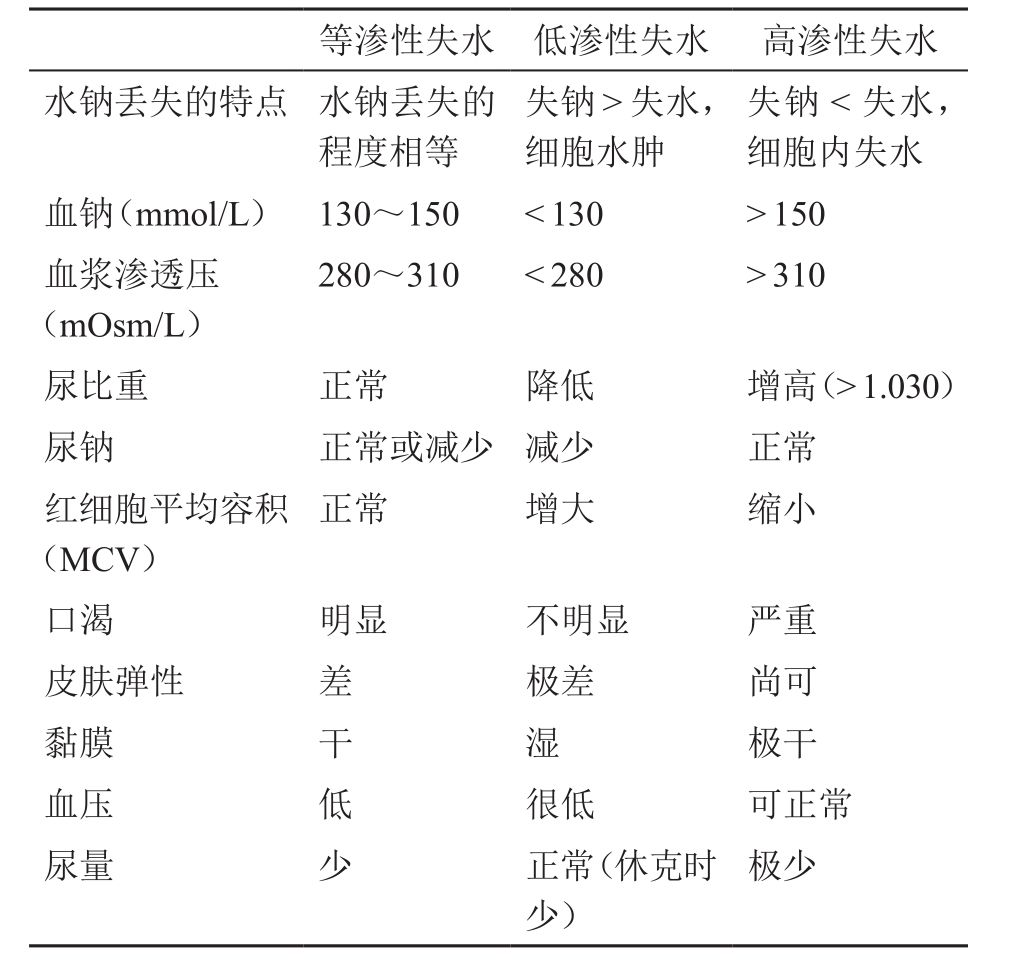
\includegraphics[width=3.40625in,height=3.20833in]{./images/Image00239.jpg}
\end{table}

\hypertarget{text00190.htmlux5cux23CHP6-1-1-3-2-1-3}{}
(3) 按血细胞比容(Hct)计算:

适用于低渗性失水的估计。需补液量(ml)=(患者Hct
−正常Hct)÷正常Hct(男为48\%,女为42\%)×千克体重× 200。

\paragraph{补液种类}

轻度失水一般补充0.9\%氯化钠液或林格液,通过机体的调节能力,水与电解质失调即可矫正。中度以上失水则需依失水的不同类型、补不同液体。一般来说,高渗性失水补液中含钠液体约占1/3,等渗性失水补液中含钠液体约占1/2,低渗性失水补液中含钠液体约占2/3。

\hypertarget{text00190.htmlux5cux23CHP6-1-1-3-2-2-1}{}
(1) 高渗性失水:

以补水为主,补钠为辅,适当补充钾及碱性溶液。经口、鼻饲者可直接补充水分,经静脉者,初始补5\%葡萄糖液,以后如血钠下降,尿比重降低,可适当补充5\%葡萄糖氯化钠液;渗透压升高明显者,初时可用0.45\%低渗氯化钠液。

\hypertarget{text00190.htmlux5cux23CHP6-1-1-3-2-2-2}{}
(2) 等渗性失水:

以补充等渗性溶液为主。0.9\%氯化钠溶液为首选,但长期使用可引起高氯性酸中毒。下述配方更符合生理需要:0.9\%氯化钠液1000ml
+ 5\%葡萄糖液500ml + 5\%碳酸氢钠液100ml。

\hypertarget{text00190.htmlux5cux23CHP6-1-1-3-2-2-3}{}
(3) 低渗性失水:

以补充高渗溶液为主。可用0.9\%氯化钠液1000ml加10\%葡萄糖液250ml及5\%碳酸氢钠100ml配成的溶液静滴,此时每1000ml液体含钠158mmol,氯113mmol,碳酸氢根44mmol。重度缺钠致血钠<
120mmol/L时,可按kg体重计算补钠:应补氯化钠(g)=(142
−血钠)×体重(kg)× 0.2 ÷
17(1g氯化钠含17mmol钠,故除以17折算为氯化钠量)。可小心静滴3\%~5\%氯化钠液。一般先补给补钠量的1/3~1/2,且不能过快,一般以血钠每小时升高0.5mmol/L为宜。

\paragraph{补液一般原则与注意事项}

①轻度失水或经静脉输液后好转者,以口服或鼻饲补液为首选;中度失水常需辅以静脉补给;重度失水则必须从静脉补给。②补液速度先快后慢,中、重度失水一般在开始4~8小时内输入补液总量的1/2~1/3,余1/2~2/3在24~48小时内补足,并根据病情的轻重、缓急、年龄、心肺肾功能等情况予以调整。③在补液过程中宜注意患者神志、血压、脉搏、呼吸、皮肤弹性、黏膜干湿度、尿量、吐泻量、及实验室检查结果等情况,作为衡量疗效的指标,调整补液量、速度与溶液的性质。并记录24小时出入水量。④急需大量快速补液时,宜口服或鼻饲补液;经静脉补充时宜监测CVP(<
12cmH\textsubscript{2}
O为宜)。⑤宜在尿量增至30~40ml/h后补钾,一般浓度为3g/L,当尿量>
500ml/d时,日补钾量可达10~12g。⑥纠正酸碱平衡紊乱。⑦补足液体的客观指标:精神好转;皮肤弹性恢复,血管充盈;舌面由干燥变成湿润;脉搏有力,呼吸均匀;血压趋于正常;补液3~4小时后尿量开始增加,如达到正常范围(40ml/h)以上者,提示补液适当,失水基本纠正。

\protect\hypertarget{text00191.html}{}{}

\section{水过多与水中毒}

水过多(water
excess)是水在体内过多潴留的一种病理状态。若过多的水进入细胞内,导致细胞内水过多则称为水中毒(water
intoxication)。水过多与水中毒是稀释性低钠血症的病理表现。

\subsection{病因与发病机制}

多因水调节机制障碍,而又未限制饮水或不恰当补液引起。

\paragraph{抗利尿激素(ADH)过多}

①ADH代偿性分泌增多:如急性外伤、大手术、失血、严重感染后、胸腔肿瘤压迫大静脉、心功能不全、药物刺激(如氯磺丙脲、环磷酰胺、巴比妥类)导致ADH释放增多;其特征是毛细血管静水压升高和(或)胶体渗透压下降,总容量过多,有效循环容量减少,体液积聚在“第三间隙”。②ADH不适当的分泌过多:如恶性肿瘤(肺癌、胰腺癌等)、肺炎、肺脓肿和脑炎、脑卒中等脑部疾病以及甲低等病者可发生ADH分泌过多;其特征是体液总量明显增多,有效循环血容量和细胞内液增加,血钠低,一般不出现水肿。③ADH用量过多:如治疗尿崩症时。

\paragraph{肾排水功能不良}

最常见于急性肾功能衰竭少尿期,过多地输液试图增加尿量而发生水中毒。

\paragraph{肾上腺皮质功能减退}

皮质醇分泌不足,使肾小球滤过率降低,对ADH抑制作用减弱,以及肾小管对ADH的敏感性改变,因而导致水潴留。

\paragraph{入水过多}

中枢神经病变刺激口渴中枢而致饮水过多,先天性巨结肠患者接受积极的灌肠治疗等可致水过多。

由于ADH分泌过多,水分未能排出而发生水过多,特别是心力衰竭、肝硬化腹水和肾病综合征的患者,有效血容量下降,引起醛固酮增多症,故使水钠潴留更为严重。水过多时首先影响到细胞外液,使细胞外液量增多,钠含量下降,呈低渗状态。当肾脏排水不良时,水分向细胞内转移,引起细胞内水过多,使细胞内外的渗透压均下降,导致细胞代谢和功能紊乱,所出现的各种症状,取决于水在体内潴留和渗透压改变的程度和速度。其中最严重者可出现脑水肿及脑疝的表现。

\subsection{诊断}

\subsubsection{具有水过多的病因存在}

\subsubsection{临床表现特点}

\paragraph{急性水过多与水中毒}

发病急,突出表现为低渗状态所致精神神经症状:头痛、视力模糊、定向力不清、精神失常、共济失调、癫痫样发作、昏迷。脑细胞水肿时出现颅内高压症,发生脑疝可致呼吸、心跳停止。

\paragraph{慢性水过多与水中毒}

起病缓慢,因常与原发病如心力衰竭、肝硬化腹水、肾病综合征等混杂在一起,故轻症很难识别,但体重常增加。当血浆渗透压≤260mOsm/L(血钠≤125mmol/L)时,有疲倦、表情淡漠、恶心、食欲减退等表现和皮下组织肿胀;当血浆渗透压降至240~250mOsm/L(血钠115~120mmol/L)时,出现头痛、嗜睡、神志错乱、谵妄等神经精神症状;当血浆渗透压降至230mOsm/L(血钠110mmol/L)时,可发生抽搐或昏迷。血钠在48小时内迅速降至108mOsm/L以下可致神经系统永久性损伤或死亡。

\subsubsection{实验室检查}

血浆渗透压与血钠明显降低;尿钠增多;血清K\textsuperscript{+}
、Cl\textsuperscript{−}
及血浆白蛋白、血红蛋白、平均红细胞血红蛋白浓度(MCHC)、血细胞比容等均降低;红细胞平均容积(MCV)增大。

\subsection{治疗}

\subsubsection{积极治疗原发病、控制水入量}

治疗原发病,去除导致ADH过多的因素,严格控制入水量是治疗的基本措施。以限制在每日700~1000ml为宜,有效指标为每日体重下降0.2~0.5kg。轻症患者使水代谢呈负平衡,即可逐渐自行恢复。

\subsubsection{急性重度水中毒}

保护心、脑功能,纠正低渗状态(如利尿脱水)。

\paragraph{高容量综合征}

以脱水为主,减轻心脏负荷。首选呋塞米、依他尼酸等袢利尿药,如呋塞米20~60mg口服,每天3~4次;急重者用呋塞米40~80mg静注,6~8小时一次。危急病例可采取血液超滤治疗,疗效确切、迅速。用硝普钠、硝酸甘油等保护心脏,减轻其负荷。明确为ADH不适当分泌过多者,除病因治疗外,可选用利尿剂、地美环素(去甲金霉素,0.9~1.2g/d,分3次口服)或碳酸锂治疗。

\paragraph{低渗血症(特别是已出现神经精神症状者)}

立即用3\%~5\%氯化钠溶液静滴,以迅速纠正细胞内液的低渗状态。一般剂量为5~10ml/kg体重,分3次静滴,开始1小时内滴入1/3量,观察1小时根据病情再考虑第2、3次的输入。5\%氯化钠液含钠855mmol/L,每升可以从细胞内液抽出6000ml水,可使血容量急骤增加而导致心力衰竭。一般于3小时内用量不宜超过250ml,并应密切监护血压、脉搏、颈静脉充盈、肺底啰音、水肿及中心静脉压、尿量、血钠等改变。一般补至脑水肿、球结膜水肿消失即可,不要求血钠达到正常水平。当血容量过多,出现心肺功能不全时,需并用呋塞米、依他尼酸以减少过多的血容量。纠正低钾、酸中毒等。

\protect\hypertarget{text00192.html}{}{}

\section{低钠血症}

低钠血症(hyponatremia)指血钠<
135mmol/L而言,仅反映钠在血浆中浓度的降低,并不一定表示体内总钠量的丢失,总体钠可正常或稍有增加。包括:①缺钠性低钠血症,即低渗性失水,体内的总钠量和细胞内钠减少,血清钠浓度降低;②稀释性低钠血症,即水过多,血钠被稀释,总钠量可正常或增加,细胞内液和血清钠浓度降低;③特发性低钠血症(消耗性低钠血症),见于各种慢性消耗性疾病如肺癌、肝硬化晚期严重营养不良、年老体衰、肺结核等。可能是细胞内蛋白质分解消耗,细胞内渗透压降低,水由细胞内移向细胞外所致。④转移性低钠血症,少见。机体缺钠时,钠从细胞外移入细胞内。总体钠可正常,细胞内液钠增多,血清钠浓度降低。前两种类型的诊断与治疗分别见上述。特发性低钠血症除原发病表现外,缺钠本身无症状,血钠降低亦轻,治疗主要针对原发病与支持疗法。转移性低钠血症少见,临床上主要表现为低钾血症,治疗以去除原发病和纠正低钾血症为主。对严重高脂血症、高蛋白血症等可引起“假性低钠血症”,主要应针对原发病因治疗。

\protect\hypertarget{text00193.html}{}{}

\section{高钠血症}

高钠血症(hypernatremia)指血清钠>
145mmol/L。可见于机体总钠量增多、正常或减少。包括:①浓缩性高钠血症:即高渗性失水,是引起高钠血症的主要原因。见高渗性失水。②潴钠性高钠血症:常见于心力衰竭、肝硬化腹水、肾病综合征及皮质醇、醛固酮增多,特别是给钠过多时。其本质是肾排钠减少,水钠潴留,但潴钠>潴水,故细胞外液量增加,甚至水肿。潴钠性高钠血症以神经精神症状为主要表现,病情轻重与血钠升高的速度和程度有关。初期症状不明显,随着病情发病或在急性高钠血症时,主要呈脑细胞失水表现,如神志恍惚、烦躁不安、抽搐、惊厥、癫痫样发作、昏迷乃至死亡。③特发性高钠血症:由口渴中枢障碍或精氨酸血管加压素(AVP)调节异常引起,病因不明。少部分病例可有脑肿瘤、肉芽肿等病变或创伤、脑卒中等病史,确切机制不明。特发性高钠血症的症状一般较轻,常伴血浆渗透压升高。

通常根据水摄入不足、失水过多、钠摄入过多等病史可以判断高钠血症的病因。若病因不明时,测定尿渗透压将有助于诊断。

若高钠血症伴尿渗透压>
700~800mOsm/L,提示下丘脑和肾功能无异常,高钠血症的原因可能为大量失水、钠负荷过多或渴觉障碍等。此时可测定尿钠浓度,若尿钠<
25mmol/L,提示水丢失或容量不足;若尿钠≥100mmol/L,提示高渗钠溶液输入过多。

若尿渗透压<血浆渗透压,则为中枢性尿崩症或肾性尿崩症。此时可给予外源性ADH(鼻腔吸入10μg的dDAVP或皮下注射5U
AVP)加以鉴别。若给药后尿渗透压上升超过50\%,提示为中枢性尿崩症;若尿渗透压无明显变化,提示为肾性尿崩症。

若高钠血症伴尿渗透压300~800mOsm/L,可有以下原因:①较重的中枢性尿崩症:可由于内源性ADH的释放,或容量缺乏使至肾小球集合管的液体减少,集合管水分重吸收使尿渗透压升高。随着水分的补充和高钠血症的纠正,多尿会逐渐明显。②部分性中枢性或肾性尿崩症:根据对外源性ADH的反应加以鉴别。前者尿渗透压上升超过至少50mOsm/L,而后者无变化。③渗透性利尿:渗透性利尿致高钠血症者对外源性ADH无反应。

除针对原发病的治疗外,浓缩性高钠血症的治疗参见高渗性失水的治疗。潴钠性高钠血症除限制钠的摄入外,可用5\%葡萄糖液稀释疗法或鼓励多饮水,但必须同时使用排钠性利尿药。因此类患者多有细胞外容量增高,需严密监护心肺功能,防止输液过快过多,以免导致肺水肿。也可用8\%葡萄糖液做透析疗法。氢氯噻嗪可缓解特发性高钠血症的症状。

\protect\hypertarget{text00194.html}{}{}

\hypertarget{text00194.htmlux5cux23CHP6-1-5}{}
参 考 文 献

1. 陆再英,钟南山.内科学.第7版.北京:人民卫生出版社,2008

2. 张文武.急诊内科学.第2版.北京:人民卫生出版社,2007

3. Melissa A,Robert W. Pathogenesis and management of hyponatremia. Am
J Med,2002,109:688

4. 陈灏珠 ,林果为.实用内科学.第13版.北京:人民卫生出版社,2009

\protect\hypertarget{text00195.html}{}{}

\chapter{钾代谢失调}

正常成人体内钾的总储量约为50mmol/kg体重(130~160g),在机体电解质中含量仅次于钠,其中3/4存在于肌肉组织。钾的分布特点是98\%在细胞内,是人及动物细胞内含量最多的阳离子,而细胞外液仅占2\%,致使细胞内K\textsuperscript{+}
浓度平均高达140~150mmol/L,而细胞外钾浓度仅是它的1/30。血清钾浓度正常介于3.5~5.5mmol/L。细胞间液为3.0~5.0mmol/L。人体钾的来源全靠从外界摄入,肉类、水果、蔬菜等均含钾丰富。每日摄入量50~75mmol,一般膳食每日可供钾50~100mmol(2~4g),足够维持生理上的需要。90\%由小肠吸收,80\%~90\%经肾脏排泄,余下10\%经粪便排出。皮肤通常排钾甚少,约5mmol/L,但大量出汗可排出较多量钾。平时,肾脏是排钾和调节钾平衡的主要器官。

钾在人体的主要生理作用是:①维持细胞的正常代谢;②维持细胞内容量、离子、渗透压及酸碱平衡;③维持细胞膜的应激性;④维持心肌的正常功能。而细胞内外钾浓度明显差异的维持与Na\textsuperscript{+}
-K\textsuperscript{+} -ATP酶的正常运转有关:Na\textsuperscript{+}
-K\textsuperscript{+}
-ATP酶可以利用ATP水解所获得的能量将细胞内的3个Na\textsuperscript{+}
转运到细胞外;同时,细胞外3个K\textsuperscript{+}
被交换到细胞内。交换而进入细胞内的1个K\textsuperscript{+}
又可通过细胞膜上的特殊通道而渗漏到细胞膜外。由于此种过程持续地进行,细胞内钾浓度可保持在相当恒定的水平,这也是形成正常细胞极化状态的原因。正常血钾水平相对恒定的维持,依靠钾的摄入、细胞内外钾的转移以及肾脏对钾排泄的调节。钾的摄入主要通过饮食,其中以水果、蔬菜含钾较多,不少软饮料中含枸橼酸钾。胰岛素、儿茶酚胺及酸碱平衡状况决定了钾在细胞内外的转移;肾小球滤过情况和醛固酮的水平则决定了肾脏中钾的排泄。胰岛素可以激活Na\textsuperscript{+}
-K\textsuperscript{+} -ATP酶,从而促使K\textsuperscript{+}
从细胞外转移到细胞内,主要为横纹肌、肝脏、脂肪等细胞;而血K\textsuperscript{+}
水平升高本身还可以刺激胰岛素分泌,进而反馈调节血K\textsuperscript{+}
水平。儿茶酚胺通过兴奋β\textsubscript{2}
肾上腺素能受体使K\textsuperscript{+}
转移到细胞内。酸中毒(主要是无机盐造成的酸中毒)使K\textsuperscript{+}
从细胞内转移到细胞外,血K\textsuperscript{+}
浓度上升;碱中毒时正好相反。从肾小球滤过的K\textsuperscript{+}
几乎100\%在近端肾小管、髓袢等部位完全重吸收,实际上从尿中排出的K\textsuperscript{+}
主要取决于远端肾小管,尤其集合管对K\textsuperscript{+}
的排泄。集合管主细胞是分泌K\textsuperscript{+}
的主要细胞,该处的间细胞则为重吸收K\textsuperscript{+}
的主要细胞。通常情况下主细胞基底侧有Na\textsuperscript{+}
-K\textsuperscript{+} -ATP酶,可以将K\textsuperscript{+}
从小管周围组织中逆电化学梯度转运到该细胞的胞质内;胞内的K\textsuperscript{+}
再通过管腔侧的钾通道顺电化学梯度而分泌到管腔中。管腔侧还具有K\textsuperscript{+}
-Cl\textsuperscript{−} 协同转运子,也可将K\textsuperscript{+}
分泌到管腔。盐皮质类固醇对K\textsuperscript{+}
的排泄起最关键的作用:该激素与其受体结合后,可以促使K\textsuperscript{+}
从皮质部集合管排泄。

\section{高钾血症}

高钾血症(hyperkalemia)是指血清钾浓度大于5.5mmol/L的一种病理生理状态,此时的体内钾总量可增多(钾过多)、正常或缺乏。血钾增高并不能反映全身总体钾的增加,在全身总体钾量缺乏时,血清钾亦可能增高;其他电解质亦可影响高钾血症的发生与发展。在下述情况下可造成假性高血钾(false
hyperkalemia),应予以注意:①止血带结扎时间过长,使缺血细胞中的钾释出增多;②溶血、红细胞中钾释出。在①、②中,血浆和血清钾浓度皆增高;③正常时血液凝固可释出钾,如血小板或白细胞过多,则释出钾增多,可造成假性高血钾,但此时仅血清钾增高,血浆钾浓度不变。

\subsection{病因与发病机制}

\paragraph{钾过多性高钾血症}

其特征是机体钾总量增多致血清钾过高,主要见于肾排钾减少;一般只要肾功能正常,尿量>
500ml/d,很少引起高钾血症。

\hypertarget{text00195.htmlux5cux23CHP6-2-1-1-1-1}{}
(1) 肾排钾减少:

主要见于肾小球滤过率(GFR)下降(急、慢性肾功能衰竭)和肾小管排钾减少(肾上腺皮质功能减退症、低肾素性低醛固酮症、肾小管性酸中毒、氮质血症或长期使用保钾利尿剂、β受体阻滞剂或血管紧张素转换酶抑制剂)。其中,急慢性肾功能衰竭是引起高钾血症最常见的原因。

\hypertarget{text00195.htmlux5cux23CHP6-2-1-1-1-2}{}
(2) 钾摄入、输入过多或过速:

含钾丰富食物(通常无钠食盐或无盐酱油中含钾量很高,每克无钠食盐含钾盐为10~13mmol,每小匙无盐酱油可含钾200mmol)或含钾溶液(如枸橼酸钾、氯化钾、青霉素钾盐、库存血)摄入或输入过多或过快,肾功能不全者更易发生。

\paragraph{转移性高钾血症}

常由细胞内钾释放或转移到细胞外所致,少尿或无尿诱发或加重病情,但机体钾总量可增多、正常或减少。包括:①细胞内钾逸出增加:如溶血、大面积组织创伤、烧伤、横纹肌溶解、淋巴瘤或白血病化疗后大量肿瘤细胞破坏、严重感染或饥饿使机体处于高分解代谢状态等,可使细胞内钾大量释出,超过肾脏的排钾能力而潴留于体内;②细胞内钾外移:如酸中毒(pH每下降0.1,血清钾可增加0.7mmol/L)、休克、高钾型周期性瘫痪、癫痫持续状态、静注精氨酸、洋地黄中毒、β受体阻滞剂等均可使细胞内钾外移。

\paragraph{浓缩性高钾血症}

重度失水、失血、休克等致有效循环血容量减少,血液浓缩而钾浓度相对升高,多同时伴有肾前性少尿及排钾减少;休克、酸中毒、缺氧等使钾从细胞内进入细胞外液。

高钾血症本身通常无特殊病理改变,但可发生肌麻痹及突然而来的严重心律失常和心搏骤停而致死亡。这是通过高血钾对细胞电生理影响所致。细胞的静息膜电位是由其内、外液钾浓度比值而决定,正常时其比值为40∶1,当血钾升高至8.0mmol/L时,比值降为20∶1。正常静息膜电位和阈电位分别为−90及−65mV,如果静息膜电位和阈电位愈接近时,细胞兴奋性愈高,但当静息膜电位明显降低,复极即受阻,因而发生肌麻痹。高血钾可降低跨膜细胞电位,始而兴奋,终至复极受阻,因而发生松弛性肌麻痹。血浆钾浓度增高对心肌细胞动作电位产生的影响是:①高血钾时,静息膜电位降低,故使0相与1相上升速度减慢,室内传导减缓,心电图(ECG)上表现为PR间期延长,QRS波增宽。②细胞膜对钾的通透性增加,此时钾较早、且较迅速地从细胞内液释出,细胞动作电位时间缩短,再极化加速,第3相下降速度加快,坡度变陡,此现象在ECG上则表现为一种尖而高的T波。由于部分去极化之故,Na\textsuperscript{+}
则不易进入细胞内,使动作电位无法正常迅速达到最高点,致使心脏去极化变慢,ECG上表现QRS波增宽,PR间期更为延长。③血钾继续增高,进而缩小细胞内、外钾浓度差,静息膜电位负值减少,从原有−90mV升至−70mV或更高,升高程度和细胞外钾浓度增加呈比例关系。当传导变慢时,心脏各部分细胞活动情形不一,可出现心室性期前收缩,严重者最后发生室性心动过速(VT),心室颤动,最后达到不能应激的地步。

\subsection{诊断}

\subsubsection{具有引起高钾血症的病因存在}

\subsubsection{临床表现特点}

\paragraph{神经肌肉系统}

早期(血清钾浓度5.5~7.0mmol/L时)常有肢体异常、麻木感觉、极度疲乏、肌肉酸痛、肢体苍白和湿冷等类似缺血现象,可能与高血钾刺激血管收缩有关。随后(血清钾浓度达7.0mmol/L以上时)出现四肢无力,尤以双下肢明显,行走困难、肌张力减低、腱反射减弱以致消失;逐渐上升至躯干肌群及双上肢,呈上升性松弛性软瘫。严重者出现吞咽、发音及呼吸困难。中枢神经系统可表现为烦躁不安、昏厥及神志不清。

\paragraph{心血管系统}

高钾血症对机体的主要危险是重症高钾血症能引起心室颤动和心搏骤停(停搏于舒张期)。高血钾对心肌细胞兴奋性、自律性、传导性以及神经(如迷走神经)的影响,加上其他电解质异常和血pH改变的参与,高钾血症对心律的影响极其复杂,可见到各种心律失常,包括各种缓慢性心律失常,如房室传导阻滞、窦性心动过缓等;也可发生快速性心律失常,如窦性心动过速、频发的室性期前收缩、室性心动过速和心室颤动等。

\paragraph{消化系统}

高血钾可使乙酰胆碱释放增加,可引起恶心、呕吐、腹痛等消化道症状。

\subsubsection{辅助检查}

\paragraph{血清钾增高}

常>
5.5mmol/L。根据血钾升高的程度,可分为三度:①轻度:血清钾5.5~6.5mmol/L;②中度:6.5~7.5mmol/L;③重度:血钾>
7.5mmol/L。

\paragraph{心电图}

高钾血症的严重程度是由测定血钾浓度和心电图变化两者共同决定的,但心电图的改变和血钾的高低无固定不变关系。一般当血清K\textsuperscript{+}
>
5.5mmol/L时,先是QT时限缩短,T波变得尖高对称,基底狭窄而呈帐篷状;至7~8mmol/L,QRS波逐渐增宽,R波振幅降低,S波加深,ST段压低,P波扁平或消失,PR间期延长,可出现窦性静止或窦房阻滞,或表现为交界区性或室性自主心律;至9~10mmol/L时,增宽的QRS波群与T波融合而呈正弦状波,出现室扑或室颤,以致心脏停搏。心电图检查时应注意碱中毒、心室肥大、心肌缺血、心包炎、洋地黄中毒、束支传导阻滞可使高钾血症的心电图变化被掩盖;低血钙、低血钠、酸中毒可加重心电图的高钾表现;高血镁可产生类似高钾的心电图变化。

\subsubsection{注意事项}

高钾血症的诊断首先要除外由于溶血等原因所致的假性高钾血症,并除外实验室误差。确定高钾血症诊断后,还要寻找和确定导致高钾血症的原发疾病。心电图检查明确有无严重的心脏毒性的发生,ECG若有高钾血症的表现是危险的信号,应采取积极的治疗措施。药物(包括钾盐)及各种病因引起的肾功能不全是最常见的导致高钾血症的原因。肾功能正常但伴严重肾前性氮质血症的患者可伴高钾血症。醛固酮、胰岛素分泌或作用的缺陷也可导致高钾血症。在初诊为肾上腺皮质功能不全的患者中40\%伴有高钾血症。持续性高钾血症伴酸中毒可能是高钾性肾小管酸中毒,常见于中度肾功能不全,尤其是伴有糖尿病、间质性肾炎或梗阻的患者。

\subsection{治疗}

高钾血症的治疗原则是迅速降低血钾水平,保护心脏。治疗措施包括以下几方面:①注射钙剂以对抗K\textsuperscript{+}
的心脏毒性;②将细胞外K\textsuperscript{+}
暂时转移至细胞内;③将K\textsuperscript{+} 清除至体外。同时须除去病因。

\subsubsection{病因治疗}

1.积极治疗原发病
如纠正酸中毒、休克,有感染或组织创伤应及时使用抗生素及彻底清创。

2.应立即停用含钾药物
、保钾利尿剂,少进含钾的食物;给予高糖高脂肪饮食以保证足够的热量,以减少分解代谢所释放的钾。避免应用库存血。

\subsubsection{重度高钾血症的治疗}

应采取紧急降低血钾浓度的措施,并自始至终都要严密监护,使血钾浓度及心律恢复至安全范围。应注意的是,当血钾未达到重度高钾血症水平,但ECG已有典型高钾表现;或者有高钾所致的典型神经肌肉症状时,也必须进行紧急处理。

\paragraph{静脉注射钙剂}

当高血钾引起心室自身节律时,应立即注射钙剂以对抗其心脏毒性。因为高血钾可使静息膜电位降低而阈电位则无变化,两者间差距减少,使心肌细胞兴奋性增加;钙离子并不能影响细胞内、外K\textsuperscript{+}
的分布,但却可使静息膜电位与阈电位间差距增加,心脏兴奋性因而较为稳定,这种治疗并不限于低血钙患者,只要患者有严重心律失常,即使血钙正常,也应立即注射钙剂。钙离子疗效相当迅速。当发现患者有严重心律失常时,应立即在心电监护下用10\%葡萄糖酸钙10~20ml加入25\%~50\%葡萄糖溶液10~20ml中,静脉缓慢(5~10分钟)注射,在数分钟内即可见效,维持约30~60分钟。注射后10~20分钟内如无效或有效后又再发生心律失常,可重复注射。也可在有效后用2~4g葡萄糖酸钙加入10\%葡萄糖1000ml内静滴维持。氯化钙含钙量为葡萄糖酸钙的4倍,如同时存在严重低钙血症者,应选用氯化钙。应注意:钙离子仅是暂时对心脏有对抗钾的毒性,并不能减低血钾浓度,仅是一种短时的急救药物,尚需采用其他措施来降低血钾。有心力衰竭者不宜同时应用洋地黄。

\paragraph{碱性药物}

可用5\%碳酸氢钠液或11.2\%乳酸钠60~100ml于10分钟内静脉注射或快速静滴,用后5~10分钟起作用,30分钟内改善症状,疗效维持数小时。注射后若无严重的碱中毒可重复使用或用上述碱性溶液100~200ml以15~30滴/分钟速度静滴维持。与葡萄糖酸钙须分别应用。待心电图恢复后,即可减量或停用。碱性药物作用有:①可碱化细胞外液,使K\textsuperscript{+}
迅速从细胞外液移入细胞内。血HCO\textsubscript{3} \textsuperscript{−}
每增高1mmol/L,血钾可降低0.13~0.18mmol/L。②Na\textsuperscript{+}
拮抗钾对心肌的毒性作用。③增加远端小管中钠含量和Na\textsuperscript{+}
-K\textsuperscript{+} 交换,使钾从尿中排出增加。④Na\textsuperscript{+}
增加血浆渗透压,扩容,起到稀释性降低血钾作用。⑤Na\textsuperscript{+}
有抗迷走神经作用,可提高心率。在房室传导阻滞时,乳酸钠可使PR时间缩短,心房及心室率加快。应注意:短期内输液量过多及输入过多的钠离子易诱发肺水肿,尤其是心肾功能不全患者,更应注意。此外,少数患者由于注射后快速产生碱血症,可诱发抽搐或手足搐搦症,此时可同时注射钙剂以对抗。

\paragraph{高渗葡萄糖及胰岛素}

静注25\%~50\%葡萄糖液60~100ml,同时皮下注射胰岛素10U或在10\%葡萄糖液500ml中,按3~4g葡萄糖用1U的比例加入胰岛素静滴,可使钾转入细胞内。注射开始后30分钟内起效,持续时间4~6小时。通常应用上述剂量后血钾可下降0.5~1.2mmol/L,必要时6小时后再重复一次。

\paragraph{高渗盐水}

其作用机制与乳酸钠相似。常用3\%~5\%氯化钠液100~200ml静滴,效果迅速,应监护心肺功能。若尿量正常,也可用等渗盐水。

\paragraph{排钾治疗}

以上措施是短效应的急救治疗,若高血钾持续存在,危及患者生命,随后须采取排钾治疗。有以下方法:

\hypertarget{text00195.htmlux5cux23CHP6-2-1-3-2-5-1}{}
(1) 利尿剂:

选用排钾利尿剂,如呋塞米、布美他尼和噻嗪类,仅适用于肾功能较好者。如用呋塞米40~120mg静注。

\hypertarget{text00195.htmlux5cux23CHP6-2-1-3-2-5-2}{}
(2) 肠道排钾:

可用阳离子交换树脂经消化道排钾。常用的为聚苯乙烯磺酸钠交换树脂10~20g口服,每天2~3次;可单独或并用25\%山梨醇20ml口服,每天2~3次。亦可用树脂40~50g置于25\%山梨醇100~200ml中,保留灌肠,每日2~3次。树脂能在肠道吸附钾而释放出钠,每克树脂约能除去1mmol钾。降钾树脂的起效时间,口服约1~2小时,灌肠为4~6小时。每50g降钾树脂大约可使血钾下降约0.5~1.0mmol/L。含钠树脂最大缺点是使过多钠离子吸收,在排水钠有障碍的患者易致水肿及心力衰竭,可选用含钙离子树脂。

\hypertarget{text00195.htmlux5cux23CHP6-2-1-3-2-5-3}{}
(3) 透析疗法:

为最快和最有效方法。尤适用于肾功能衰竭伴高钾血症者。可行血液或腹膜透析治疗,但血透常比腹透更有效。应用低钾或无钾透析液进行血透,可以使血钾几乎在透析开始后即下降,1~2小时后血钾几乎可恢复到正常。腹透应用普通标准透析液在每小时交换2L情况下,大约可交换出5mmol钾,连续透析36~48小时可以去除180~240mmol钾。

若高血钾有危及生命的心律失常,应紧急安置静脉插管临时起搏,并迅速准备行透析治疗,度过高血钾期。

\subsubsection{中度高钾血症的治疗}

必须立即注射葡萄糖、胰岛素及碳酸氢钠液,使钾离子尽快转移入细胞内,降低血钾浓度,同时去除病因。

\subsubsection{轻度高钾血症的治疗}

通常只减少钾盐的摄入,停用或减少钾离子含量丰富的药物,进低钾饮食,除去血钾增高的原因等。

\protect\hypertarget{text00196.html}{}{}

\section{低钾血症}

低钾血症(hypokalemia)是指血清钾<
3.5mmol/L的一种病理生理状态。其中,血K\textsuperscript{+}
在3.0~3.5mmol/L之间称为轻度低钾血症,症状较少;血K\textsuperscript{+}
在2.5~3.0mmol/L之间为中度低钾血症,可有症状;血K\textsuperscript{+} <
2.5mmol/L为重度低钾血症,出现严重症状。

\subsection{病因与发病机制}

\paragraph{缺钾性低钾血症}

表现为体内总钾量、细胞内钾和血清钾浓度降低。①摄入钾不足:见于长期厌食、偏食、禁食以及静脉补液内少钾或无钾者。每日钾的摄入量<
3g,并持续2周以上。②排出钾过多:主要是经肾或胃肠道失钾。肾脏失钾是低钾血症最常见原因,其诊断标准为尿钾排泄>
20mmol/d且无腹泻病史。例如:长期应用排钾利尿剂;各种以肾小管功能障碍为主的肾脏疾病;长期应用肾上腺皮质激素或肾上腺皮质功能亢进,尤其是醛固酮增多症。

\paragraph{转移性低钾血症}

表现为体内总钾量正常、细胞内钾增多和血清钾浓度降低。见于:①注射大量葡萄糖液(特别是同时应用胰岛素时):在葡萄糖进入细胞合成糖原过程中,大量钾离子移入细胞内(合成1g糖原约需0.15mmol钾)。②碱中毒时,钾离子进入细胞内与H\textsuperscript{+}
交换,血pH每增高0.1,可使血清钾降低0.7mmol/L。③酸中毒的恢复期。④周期性瘫痪发作期。⑤棉籽油或氯化钡中毒。⑥低温疗法使钾进入细胞内。

\paragraph{稀释性低钾血症}

表现为体内总钾量和细胞内钾正常,血清钾浓度降低。见于水过多和水中毒,或过多过快补液而未及时补钾时。

缺钾时细胞内外Na\textsuperscript{+} 、K\textsuperscript{+}
产生相互转移,通常是3个K\textsuperscript{+}
从细胞内向外移,而有2个Na\textsuperscript{+} 和1个H\textsuperscript{+}
进入细胞内,以调整细胞内外的电解质成分。血钾减少时心肌细胞膜静息电位增大,动作电位时间延长,反映在ECG上为进行性ST段压低、T波振幅减少,U波出现与增大。T波可降低转为平坦,最后转成双相、倒置。U波常超过同导联T波高度,TU可融合成驼峰样。低血钾心肌细胞对K\textsuperscript{+}
的通透性降低,Na\textsuperscript{+} 流入超过K\textsuperscript{+}
流出,使细胞内电位的负性减少,起搏细胞的自律性增加。并可抑制心肌传导及产生异位激动,导致各种心律失常,主要为房性、房室交接处或室性过早搏动,大多发生在前一心动周期的U波上,呈多形性、多源性,并转为室颤前的室性心动过速,以致出现心搏骤停。也可出现房室传导阻滞。

当血清K\textsuperscript{+} <
3.0mmol/L时可出现肌无力,血清K\textsuperscript{+}
<2.5mmol/L时可以出现软瘫。肌无力的发生机制可能是通过细胞内、外钾的比例改变,而使细胞超极化。由于静息电位与阈电位远离,而致兴奋性降低,对Ach的兴奋反应性减低。

\subsection{诊断}

\subsubsection{有低钾血症的病因存在}

\subsubsection{临床表现特点}

低钾血症的临床表现取决于低血钾发生的速度、程度和细胞内外钾浓度异常的轻重。慢性轻度低钾血症的症状轻或无症状,而迅速发生的重度低钾血症往往症状很重,甚至引起猝死。

\paragraph{神经肌肉系统}

一般血清钾< 3.0mmol/L时,患者感疲乏、软弱、乏力;<
2.5mmol/L时,全身性肌无力,肢体软瘫,腱反射减弱或消失,甚而膈肌、呼吸肌麻痹,呼吸困难、吞咽困难,严重者可窒息。常伴有肌肉酸痛、麻木感、感觉异常和手足搐搦。

\paragraph{中枢神经系统}

轻者表现为倦怠、精神不振;重者反应迟钝、定向力丧失、精神错乱、意识障碍、昏迷。

\paragraph{消化系统}

恶心、呕吐、食欲不振、腹胀、便秘,严重者肠麻痹等。

\paragraph{心血管系统}

低钾血症对心脏的主要影响为心律失常。轻度低血钾多表现窦性心动过速、房性及室性期前收缩;重度低血钾可致室上性或室性心动过速及室颤等严重心律失常,偶可发生房室传导阻滞。此外,心肌的损害可有第一心音减弱、心脏扩大、心动过速、心力衰竭等。血管平滑肌的麻痹可致血压下降、休克。

\paragraph{泌尿系统}

长期低钾可引起失钾性肾病和肾功能障碍,浓缩功能减退,出现多尿、夜尿、口渴、多饮,尿比重低,尿中有少量蛋白和管型。

\paragraph{代谢紊乱}

大量长期失钾,Na\textsuperscript{+} 和H\textsuperscript{+}
进入细胞内引起细胞内酸中毒,细胞外碱中毒,且由于氯的排出增多,易形成低钾低氯性碱中毒。血清钙可正常、降低或增高。低血钾可使糖耐量减退。血清钾降低常能反映细胞内缺钾情况。血钾下降1mmol/L,体内丢钾约100~200mmol,当血清钾在3.0mmol/L以下时,每下降1mmol/L,体内丢钾约200~400mmol;当心电图出现U波时,往往提示体内丢钾至少500mmol。

\subsubsection{辅助检查}

\paragraph{血清钾测定}

血清钾< 3.5mmol/L为低钾血症。严重低血钾(<
2.5mmol/L)常伴有代谢性碱中毒致CO\textsubscript{2}
CP、血pH、标准碳酸氢盐(SB)升高,但尿呈酸性。

\paragraph{心电图检查}

T波低平、双相或倒置;U波出现并逐渐增高,常超过同导联的T波,T波与U波相连呈驼峰状,QT间期延长,P波振幅增高,PR间期延长。以胸前导联V\textsubscript{2}
、V\textsubscript{3} 较明显。应注意:血pH、HCO\textsubscript{3}
\textsuperscript{−} 、Na\textsuperscript{+}
等升高时也可产生类似的心电图改变,其他电解质尤其是Ca\textsuperscript{2+}
也有影响,要注意鉴别。

\subsubsection{诊断注意事项}

低钾血症患者需进行详细的病史采集、体格检查及实验室检查,以明确低钾的原因。首先应除外由异常白细胞摄取钾所造成的假性低钾血症;其次,是否有激素、药物或其他导致钾从细胞外转移至细胞内的因素存在。若以上均可除外,则低钾血症血钾从肾脏、胃肠道及皮肤丢失所引起。此时,尿钾测定有助于判断病因。肾外失钾(胃肠道、皮肤等)尿钾一般<
15mmol/L,>
20mmol/L则多表示经肾丢失,其中最常见的为利尿剂的使用,其他原因还有肾小管酸中毒(RTA)、糖尿病酮症酸中毒以及输尿管乙状结肠吻合术后等。如疑为原发性醛固酮增多症,要测定血浆肾素活性和醛固酮水平。

\subsection{治疗}

积极治疗原发病,给予富含钾的食物。对缺钾性低钾血症者,除积极治疗原发病外,还应及时补钾。

\paragraph{补钾量}

参照血清钾水平,大致估计补钾量。血清钾3.0~3.5mmol/L,可补充钾100mmol(相当于氯化钾8.0g);血清钾2.5~3.0mmol/L,可补充钾300mmol(相当于氯化钾24g);血清钾2.0~2.5mmol/L水平,可补充钾500mmol(相当于氯化钾40g)。包括口服补钾量在内。但一般每日补钾以不超过200mmol(15g氯化钾)为宜。

\paragraph{补钾种类}

最好是饮食补钾。肉、青菜、水果、豆类含钾量高,100g约含0.2~0.4g,而米、面约含钾0.09~0.14g,蛋约含钾0.06~0.09g。药物补钾:①氯化钾(1g
=
13.4mmol钾):最常用。②枸橼酸钾(含钾约9mmol/g)。③醋酸钾(含钾约10mmol/g)。枸橼酸钾和醋酸钾适用于伴高氯血症者(如肾小管性酸中毒)的治疗。④谷氨酸钾(含钾约4.5mmol/g),适用于肝衰竭伴低钾血症者。⑤L-门冬氨酸钾镁溶液:含钾3.0mmol/10ml,镁3.5mmol/10ml,门冬氨酸和镁有助于钾进入细胞内。

\paragraph{补钾方法}

轻者鼓励患者进食含钾丰富的水果、蔬菜和肉类。口服补钾以氯化钾为首选,每日3~6g(1g
=
13.4mmol钾)。为减少胃肠道反应,宜将10\%氯化钾溶液稀释于果汁或牛奶中餐后服,或用氯化钾控释片,或换用枸橼酸钾,或鼻饲补钾。缺钾较重与不能口服,或出现严重心律失常、神经肌肉症状者,应静脉补钾。因患者多同时合并代谢性碱中毒,故以补氯化钾为最好。氯化钾不可静注,应溶于0.9\%氯化钠液或5\%葡萄糖液内静滴。可用10\%氯化钾15~30ml加入0.9\%氯化钠液1000ml(钾浓度相当于20~40mmol/L),静脉滴注。静脉补钾时,钾浓度不宜超过40mmol/L(即0.3\%氯化钾),速度以20~
40mmol/h为宜(即氯化钾1.5~3.0g/h),不能超过50~60mmol/h。一般每日40~80mmol(相当于氯化钾3~6g),第1日可用80~134mmol(相当于氯化钾6~10g)。对因缺钾发生严重心律失常、呼吸肌麻痹危及生命时,补钾量可增大,速度可加快:可用10\%氯化钾50~100ml加入0.9\%氯化钠液1000ml中,在持续心电监护和严密监测血钾下,以30~50mmol/h的速度静滴,直至血钾浓度达到或接近3.0mmol/L。也可采用精确的静脉微量输注泵以较高浓度的含钾液体行深静脉穿刺或插管微量匀速输注。对钾缺乏而合并酸中毒或不伴低氯血症者,可用谷氨酸钾液20ml加入5\%葡萄糖500ml静滴。

\paragraph{补钾注意事项}

①在静脉补钾过程中,需密切监测心电图和血清钾,每2小时测血钾1次{[}在高浓度和(或)快速静脉补钾时,至少1小时测血钾1次{]},以防突然产生高钾血症而发生心搏骤停,有条件应作连续心电监护。②见尿补钾:在血容量减少、周围循环衰竭、休克致肾功能障碍时,除非有严重心律失常或呼吸肌麻痹等紧急情况,应待补充血容量、排尿达到30~40ml/h后,继续观察6小时,开始予补钾。一般尿量达500ml/d以上可予以补钾。③钾进入细胞内较为缓慢,完全纠正需4~6天,故不宜过多过快静脉补钾,以免发生高钾血症。经过2~3天病情好转后,宜逐渐减量,或改为口服,但不可骤然停药。氯化钾对胃肠道刺激性大,长期应用有引起小肠溃疡、出血、穿孔的危险。④对难治性低钾血症,应注意是否合并碱中毒或低镁血症,纠正碱中毒及补充镁后,低钾血症可迅速纠正。⑤低钾血症与低钙血症并存时,低钙血症症状常不明显,补钾后有时可出现手足搐搦或痉挛,应补充钙剂。⑥低血钾患者如静脉滴注葡萄糖加胰岛素或碳酸氢钠,可加重低血钾,因而非必要时不宜采用,必须用时,应同时补钾。

\protect\hypertarget{text00197.html}{}{}

\chapter{镁代谢失调}

镁是人体必需元素之一。细胞内的阳离子中镁的含量仅次于钾。镁广泛存在于体内各组织中,参与许多生物学过程,尤其是对酶的活性、能量代谢及神经肌肉传递方面起着重要作用。正常成人体内镁的总储量约1000mmol(24g),其中50\%~60\%存在于骨骼中,40\%~60\%存在于软组织中,细胞外液中的镁离子仅占总量的1\%。正常人血镁浓度为0.75~1.25mmol/L,以三种形式存在:①游离镁:约占55\%以上,正常值为0.52(0.46~0.57)mmol/L;②结合镁:系镁与重碳酸根、磷酸根和枸橼酸根等所形成的复合物,约占15\%,正常值为0.14mmol/L;③蛋白结合镁:约占30\%,正常值为0.2~0.3mmol/L。人类每日每千克体重需要摄入镁0.15~0.18mmol才能维持正常平衡,日常镁摄取量的2/3以上来自绿叶蔬菜和粮食,其余来自肉和乳类。摄入后有30\%~50\%被吸收,部位以空肠、回肠为主。经肠道吸收的镁大部分经肾排出,小部分经胆汁、胰液及肠液分泌入肠道。人体镁代谢的内平衡主要是依靠肠道吸收和肾脏排泄镁的调节而完成的,但下列因素对其有重要影响:①甲状旁腺激素(PTH):具有增加肠道吸收和促进肾近曲小管重吸收镁的作用,并通过负反馈机制参与血清镁浓度的调控;②甲状腺素:能促进肠道吸收镁,但又能直接抑制肾小管重吸收镁,使尿镁排泄量显著增加;同时,它能促进全身代谢而增加镁的需要量。总的影响是负镁平衡,使血浆镁下降;③胰岛素:具有促进镁进入细胞内的作用,但又可使血浆磷酸盐降低,从而减少骨骼对钙、镁的摄取,其总的结果可使血浆镁升高;④醛固酮:它能减少肠道镁吸收和肾近曲小管和髓袢镁重吸收,并与其保钠作用有关,增加镁从尿和粪中的排泄,引起负镁平衡;⑤生长激素:促进肠道吸收镁,降低肾小管重吸收镁,并能促进镁进入细胞内,增加镁贮池、降低血镁浓度;⑥维生素D:可增加肠道镁的吸收;⑦Ca\textsuperscript{2+}
及磷酸盐:Ca\textsuperscript{2+} 与Mg\textsuperscript{2+}
有竞争现象;膳食中的过多磷酸盐可与Mg\textsuperscript{2+}
形成不溶解的复合物,减少Mg\textsuperscript{2+} 的吸收。

\section{低镁血症}

血清镁低于0.75mmol/L(1.82mg/dl)时称为低镁血症(hypomagnesemia)。

\subsection{病因与发病机制}

\subsubsection{病因}

\paragraph{镁摄取不足}

禁食、厌食或营养不良伴有不断的经尿排镁2个月后即可丢失体内镁总储量的1/5,主要是肌肉失镁,严重者血清镁浓度才见降低。

\paragraph{镁丢失过多}

①经胃肠道失镁:丧失消化液如持续呕吐、长期腹泻、胃肠吸引或胃肠瘘可引起镁丢失增多,而静脉只补无镁液体时;胃肠道疾患如脂肪泻、吸收不良综合征、胆道疾患与急性重型胰腺炎等。②经肾失镁:肾脏排镁过多见于各种原因引起的多尿,如长期服用髓袢及噻嗪类利尿剂,尿镁排出可增加25\%~40\%;肾小球肾炎、肾盂肾炎及肾小管性酸中毒时皆可影响肾小管对镁的重吸收功能;原发性醛固酮增多症与皮质类固醇及ACTH治疗中,肾排镁过多亦可导致低镁血症。③经透析失镁:尿毒症患者用无镁透析液透析时,也可引起低镁血症。④经皮肤失镁:重度烧伤可致低镁血症。

\paragraph{镁离子在细胞内外的重新分布}

常见原因有:①甲状旁腺功能亢进伴严重骨病的患者在甲状旁腺切除术后,过量PTH的突然清除使大量Ca\textsuperscript{2+}
和Mg\textsuperscript{2+}
进入到骨细胞内,使血镁明显下降,称为骨饥饿综合征(hungry bone
syndrome);②重症急性胰腺炎,主要因大量镁盐沉着于坏死的胰腺周围脂肪组织中;③高热能肠外营养,镁随营养物质进入细胞内供组织修复,引起血镁下降;④糖尿病酮症酸中毒,经液体和胰岛素治疗后,可使大量Mg\textsuperscript{2+}
进入细胞内而致血镁过低。

\subsubsection{病理生理}

\paragraph{对电生理的影响}

镁是许多酶的激活剂,Mg\textsuperscript{2+}
具有兴奋心肌内线粒体的氧化磷酸化作用,能影响细胞膜的Na\textsuperscript{+}
-K\textsuperscript{+} -ATP酶和激活心肌环化酶,并在K\textsuperscript{+}
和Ca\textsuperscript{2+}
的共同作用下维持细胞内外的Mg\textsuperscript{2+}
浓度,以维持正常的心肌兴奋性。在缺血性心脏病时,由于心肌缺镁,细胞氧化磷酸化过程障碍,维持细胞内钾浓度所必需的能量不足,而造成失钾,加上酶的功能障碍,钠泵衰竭,影响透膜动作电位,加重心肌的复极不一致,导致激动的差异传导和折返激动而发生心律失常。当补镁时可激活Na\textsuperscript{+}
-K\textsuperscript{+}
-ATP酶,使细胞保钾加强,心肌绝对不应期延长,且拮抗Ca\textsuperscript{2+}
的作用,影响离子膜的通透性及其结合、分布及交换,使跨膜的内向离子流减少,故能纠正心律失常。

\paragraph{对钾代谢的影响}

低镁血症时,导致低钾血症或低钾血症难纠正的可能机制是:低镁可以导致钾从髓袢及皮质部集合管分泌过多,这是因为髓袢上升支有钾分泌通道,正常时该通道被ATP所抑制,低镁时通道抑制被解除,导致钾大量分泌。

\paragraph{对神经肌肉的影响}

Mg\textsuperscript{2+}
对神经肌肉有抑制作用,当各种原因引起的血浆Mg\textsuperscript{2+}
浓度下降,使得神经肌肉接头处的Ach释放增加,使肌肉兴奋性增强引起肌肉强直性收缩,出现神经系统的症状。

\paragraph{对心肌代谢的影响}

各种原因所致的低镁血症,心肌细胞内镁缺乏,不仅是差异性传导、折返激动的电生理学基础,更为重要的是镁的不足影响了心肌代谢,降低了心肌舒缩功能。缺镁时,肌球蛋白ATP酶的活性受到抑制,分解ATP障碍,使心肌在舒缩时得不到足够的能量供应,而促发和加重心力衰竭。同时,使心肌对洋地黄高度敏感,增加了洋地黄中毒的可能性。而给镁剂可逆转洋地黄中毒引起的心律失常,在心力衰竭时补镁即能激活ATP酶和心肌腺苷环化酶,并能维持心肌线粒体的完整性,并促进其氧化磷酸化过程,进而改善心肌的代谢,增加心肌的收缩力,增加心排血量。此外镁还能扩张血管有利尿作用,从而减轻心脏的前后负荷,改善心功能,提高有效循环量。故在心力衰竭时补镁,不仅能迅速纠正心衰,减少洋地黄的用量及其中毒反应;而且能防止低血钾,避免心律失常。

\subsection{诊断}

\subsubsection{有低镁血症的病因存在}

\subsubsection{临床表现特点}

\paragraph{神经肌肉系统}

Mg\textsuperscript{2+}
对神经系有抑制作用,故缺镁时神经肌肉兴奋性增高,表现为肌肉震颤、手足搐搦、手足徐动样或舞蹈样动作、眼球震颤、反射亢进、共济失调等,上肢尤为明显。Trousseau征或Chvostek征阳性,但血钙正常。有时出现视或听觉的过敏反应。重症病例可有谵妄、精神错乱、定向力障碍、甚至幻觉、惊厥、昏迷等症状。

\paragraph{心血管系统}

表现为心悸、心动过速、快速型心律失常,半数患者有血压升高、四肢发绀等。

\paragraph{其他}

常伴有难以纠正的低钾血症和低钾性碱中毒。

\subsubsection{辅助检查}

当血清镁<
0.75mmol/L时即可诊断为镁缺乏症。但缺镁的诊断有时较困难,如有时血清镁虽在0.75mmol/L以上,仍不能否定低镁血症。血镁虽是评价镁代谢的重要指标,但因其受酸碱度、蛋白和其他因素变化的影响,不一定能反映体内镁贮备状态,也不能作为估计体内镁缺乏程度的可靠指标。若根据病史和临床判定有缺镁,而血镁正常,应作尿镁排泄量测定,如24小时尿镁排泄量<
1.5mmol,则可诊断为镁缺乏症。尿镁排泄量在补镁后可见增加。

静脉内镁负荷试验有助于诊断。正常人每千克体重给予0.125mmol镁负荷时,则负荷量的80\%以上于24小时内由尿排泄,48小时完全排除;在镁缺乏症时,负荷镁的40\%以上在体内保留。一般是在12小时内静滴含有30mmol硫酸镁的葡萄糖液500ml,然后收集24小时尿液测定尿镁排泄量,若体内有>
50\%的镁保留则为缺镁;若<
30\%可排除缺镁。也可在1~2小时内静滴含有20mmol镁的葡萄糖液400ml,收集16小时尿液测定镁含量,如为输入的20\%左右表示有缺镁,若为输入的70\%可排除缺镁。本试验在肾功能不全、心脏传导阻滞或呼吸功能不全时忌用。

\subsection{治疗}

\subsubsection{积极治疗原发病}

\subsubsection{补镁疗法}

肾脏的保镁功能较差,即使在缺镁状态下补充的镁仍有50\%可以从尿中排泄,故补充的镁量要高于推测丢失量的2倍左右。应当注意,补镁治疗要使体内镁缓慢恢复正常,一般至少需治疗4~5天以上,同时应纠正低钙和低钾血症。肾功能有损害,GFR减低时应慎重,镁用量要小,并及时监测血镁水平,以防发生镁中毒的危险。

轻度缺镁患者,可由饮食或口服补充镁剂。可用氧化镁0.5g,或氢氧化镁0.2~0.3g,或10\%醋酸镁溶液10ml,每日3~4次口服。

若患者对口服不能耐受或不能吸收时,可采用肌肉注射镁剂。第一天肌注硫酸镁2g(镁8.15mmol),每4小时1次,共5次;第2~5天肌注1g(4.1mmol),每6小时1次,共注射26g,含镁105.5mmol。如病情需要增加剂量,第一天肌注2g,每2小时1次,共3次;然后每4小时1次,共6次。第3~5天肌注1g,每6小时1次,共注射32g,含镁130mmol。肌注疗法一般采用20\%~50\%硫酸镁。

若属重度缺镁,出现严重手足搐搦、痉挛发作或室性心律失常,则须静脉滴注。常用的是硫酸镁,硫酸镁1g含镁4.07mmol。切不可用25\%~50\%的硫酸镁液静脉注射,因可发生致命性危险。首先用硫酸镁3g(12.2mmol)加入葡萄糖液1000ml中,于6小时内静滴,继以3g于2000ml溶液中缓慢静滴。第2~5天,每天给4g(16.3mmol)于溶液中静滴。如有惊厥、昏迷或严重室性心律失常,可用硫酸镁1~1.25g于50\%葡萄糖液40ml中缓慢(5~10分钟以上)静注,继以5g于1000ml溶液中于10小时静滴完毕,在以后5天内可每日补5g。静脉补镁时速度应缓慢,过快可致短暂性低血压,部分是因镁使皮肤肌肉的血管扩张所致。如静脉给予镁剂过量,可引起血压迅速下降、肌肉麻痹、呼吸衰竭和心脏停搏。若有镁剂过量,应立即静注10\%氯化钙5~10ml,必要时可重复应用。

在纠正低镁血症的同时,应纠正低血钙、低血钾、低血磷等其他电解质紊乱。

\protect\hypertarget{text00198.html}{}{}

\section{高镁血症}

血清镁浓度>
1.25mmol/L(3.0mg/dl)时称为高镁血症(hypermagnesemia)。除少数医源性因素导致进入体内镁过多外,大多是因肾脏功能障碍引起排泄减少所致。

\subsection{病因与发病机制}

\paragraph{肾排镁减少}

①急、慢性肾功能衰竭尤其是伴有少尿而又接受镁剂治疗时;②甲状腺功能减退与肾上腺皮质功能减退(甲状腺素和醛固酮可抑制肾小管镁重吸收,促进尿镁排泄)。

\paragraph{细胞内镁外流增多}

如糖尿病酮症酸中毒、外科应激反应、严重细胞外液不足及严重酸中毒等。

\paragraph{服用含镁制剂过多}

见于服用过多的含镁泻药及抗酸药,缺镁时补镁过多,用含镁制剂治疗新生儿手足搐搦症、甲亢、心律失常及洋地黄中毒等。

\paragraph{骨镁释出过多}

骨的破坏性肿瘤或恶性肿瘤骨转移时,可将骨内储存的镁释放入血,引起高镁血症。

\subsection{诊断}

1.有高镁血症的病因存在。

2.临床表现特点

(1)
神经肌肉系统:过量的镁可阻断神经传导及在末梢神经部位阻断乙酰胆碱释放,减低神经肌肉接头的冲动传导,并使突触后膜反应性降低和轴索兴奋阈值增高,从而使神经肌肉功能减低。当血清镁1.5~2.5mmol/L时,可发生恶心、呕吐;达2.5~3.5mmol/L时,可出现嗜睡、软瘫、腱反射迟钝;达3.5~5mmol/L时,可发生木僵、精神错乱、共济失调;达5~6mmol/L时出现呼吸抑制;达6~7.5mmol/L时,则可发生昏迷。

(2)
心血管系统:高镁血症可引起心脏的冲动传导障碍和抑制细胞膜的兴奋性。血清镁达1.5~2.5mmol/L时,可引起直立性低血压和心动过缓。随着血镁浓度升高,可发生心电图变化:血镁浓度2.5~5.0mmol/L时出现PR间期延长和室内传导阻滞,伴有QRS时限增宽、T波高耸和QT间期延长,P波低平。如>
7.5mmol/L时可发生完全性传导阻滞,并可抑制心脏收缩而致停搏于舒张期。

高血镁最常见于尿毒症患者,且其早期表现常与尿毒症相似而易被忽略,故在尿毒症时应加以重视。所有急性肾衰者,均应测定血镁,在慢性肾衰竭者亦最好定期检测。当肾衰患者出现神经肌肉症状及心电图示传导障碍,而不能用血钾、钙、磷异常解释时,应想到本症。由于高血镁的心电图与高血钾的相似,首先应排除高血钾的可能,才能诊断高血镁。

\subsection{治疗}

\paragraph{积极治疗原发病因}

一旦作出高镁血症的诊断,应立即停止镁制剂的摄入和治疗其原发病因。对肾功能正常者可给予强力利尿剂,以促进尿镁的排泄。

\paragraph{注射钙剂}

急性镁中毒者,应及早用10\%葡萄糖酸钙液10~20ml加等量葡萄糖静注,以拮抗高镁血症时心肌的抑制作用。如注射后5~10分钟仍未见效,应重复治疗,每日最高剂量可达10g,但须注意避免发生高钙血症。

\paragraph{透析疗法}

高镁血症最有效的疗法是血液透析,血镁下降的程度取决于透析液的离子梯度;如用无镁透析液3~4小时内即可使血镁降低。如无血透设备也可采用腹膜透析治疗。

\protect\hypertarget{text00199.html}{}{}

\chapter{钙代谢失调}

成人体内钙总量为1000~1300g,99\%左右以骨盐形成存在于骨骼中,其余存在于各种软组织中。细胞外液中钙仅占总量的0.1\%,约1g。血钙指血浆钙,测定时用血清,即血清钙,正常人血清钙为2.25~2.75mmol/L(9~11mg/dl)。含量相当稳定,儿童较高,常处于正常值的上限。血浆钙主要以三种形式存在:游离钙(离子钙,占50\%)、复合钙(与阴离子结合钙,占10\%)和蛋白结合钙(占40\%)。尿液中只有游离钙(50\%)和复合钙(50\%)。游离钙与复合钙为可扩散性,蛋白结合钙为非扩散性。非扩散性与游离钙之间常可互相转化。血浆蛋白增多时使血浆总钙量增加,但游离钙浓度不会发生改变。保持体钙贮备和最终血浆钙浓度依赖于饮食中钙摄入、肠道钙吸收和钙在粪、尿中的排泄。每日膳食摄入钙约1000mg,约400mg从食物中被吸收,200mg经胆、胰、肠排泄,净吸收为200mg。正常人粪钙排量约占摄入量的75\%~80\%,由食物中未被吸收的钙和消化液中的钙组成。尿钙约占钙摄入量的20\%。一般实验室均测定血浆钙总量,游离钙测定较困难,用钙电极测定血清游离钙浓度为1.10~1.34mmol/L。游离钙是生理活性成分,它有参与血液凝固、维持心肌节律性和收缩性,保持神经肌肉的正常兴奋性作用。细胞外钙离子浓度的恒定基两个关键因素:①感知细胞外Ca\textsuperscript{2+}
的细胞,如甲状旁腺细胞、甲状腺C细胞及肾近端小管细胞,通过细胞表面细胞外Ca\textsuperscript{2+}
感知受体(CaR)来感知细胞外Ca\textsuperscript{2+}
的细微波动,当细胞外Ca\textsuperscript{2+}
失衡时,能分别调节甲状旁腺激素(PTH)、降钙素及维生素D{[}1,25(OH)\textsubscript{2}
D\textsubscript{3} {]}三种激素的释放,使Ca\textsuperscript{2+}
趋于正常。②效应组织,如骨、肠及肾。甲状旁腺细胞、甲状腺C细胞及肾近端小管细胞通过释放激素作用于效应组织来完成调节Ca\textsuperscript{2+}
浓度。

PTH对钙的代谢有多方面的作用:①PTH激活肾小管细胞内腺苷酸环化酶,抑制肾小管磷的重吸收。磷在肾小管内有抑制1α-羟化酶的作用,而PTH可促进磷的排泄,故它能解除磷对1α-羟化酶的抑制作用,有利于维生素D的活化,使25-羟维生素D\textsubscript{3}
{[}25(OH)\textsubscript{2} D\textsubscript{3}
{]}在肾脏转变为活性更强的1,25-双羟维生素D\textsubscript{3}
{[}1,25(OH)\textsubscript{2} D\textsubscript{3}
{]},进一步促进肠钙的吸收。②能促使骨中未分化的间叶细胞分裂及转化为破骨细胞,且使破骨细胞内Ca\textsuperscript{2+}
含量增加,进而加以释放;还能把骨密质中的Ca\textsuperscript{2+}
动员出来,从而引起细胞外液的Ca\textsuperscript{2+}
浓度升高。③促进肾小管(皮质髓袢升支粗段、远曲小管、集合管等部位)对Ca\textsuperscript{2+}
的重吸收,减少Ca\textsuperscript{2+}
的排泄。④抑制肾小管对碳酸氢根及磷酸根的重吸收,增加排泄,从而解除磷酸根对PTH的拮抗及对PTH活性的抑制。此外,碳酸氢根排泄的增加,引起肾小管酸中毒,则能减少钙与蛋白质的结合,从而增加游离钙的浓度。

维生素D(胆骨化醇)是一种前激素,其活性羟化物是一种类固醇激素,名为开环类固醇,它作用于靶器官,调节钙、磷代谢。维生素D\textsubscript{3}
须先在肝细胞中羟化生成25-(OH)D\textsubscript{3}
,与血浆中α2-球蛋白结合而运转到达肾小管细胞的线粒体中再羟化,生成1,25(OH)\textsubscript{2}
D\textsubscript{3}
,成为维生素D的活性形式,分泌入血循环发挥生理作用。1,25(OH)\textsubscript{2}
D\textsubscript{3} 进入肠黏膜细胞与1,25(OH)\textsubscript{2}
D\textsubscript{3}
的受体蛋白结合后,部分转入细胞核内,影响DNA的转录过程,而促进钙结合蛋白的合成。由于钙结合蛋白对钙的亲和力大,才使肠黏膜能主动的吸收食物中的钙。它还可促进刷状缘中需钙的ATP酶合成,使ATP分解供能,增强钙的主动吸收。1,25(OH)\textsubscript{2}
D\textsubscript{3} 还能协助PTH增加肾小管对钙的重吸收,减少钙的排泄。

降钙素(calcitonin)系由甲状腺滤泡旁细胞分泌的一种激素,甲状旁腺及胸腺也可分泌少许。降钙素抑制破骨细胞的形成及其对骨的吸收,使钙质沉积于骨中,并作用于肾小管抑制对钙的重吸收,其作用在多方面与PTH拮抗。

\section{低钙血症}

血钙<
2.25mmol/L(9mg/dl)时称低钙血症(hypocalcemia)。若低于1.75mmol/L(7mg/dl)或游离钙低于0.9mmol/L
(3.6mg/dl)时,神经肌肉兴奋性增高,可发生手足搐搦症,甚至全身肌肉痉挛、抽搐、支气管哮喘、呼吸困难、心律失常、心绞痛、心力衰竭、腹痛、腹泻、癫痫样发作等,少数患者发生昏迷甚至死亡,谓之低血钙危象(crisis
of hypocalcemia)。

\subsection{病因与发病机制}

凡可造成钙的供给不足、吸收不良、调节障碍(包括PTH、降钙素分泌异常)、先天性骨和肾的细胞膜受体缺陷,对PTH完全或部分无反应,或靶组织细胞对cAMP无反应、排出过多等疾病均可诱发本症。常见的病因有:

\paragraph{甲状旁腺功能减退症}

包括原发性和继发性甲状旁腺功能减退,前者是一组多原因疾病,如先天性甲状旁腺发育不全或不发育、DiGeorge综合征、自身免疫性多腺体综合征Ⅰ型等;后者较为常见,多因甲状腺手术时误伤或切除甲状旁腺引起,也可因颈部恶性肿瘤放射治疗所并发。持续性甲状旁腺功能减退致PTH缺乏,PTH具有抑制肾小管再吸收磷,造成尿磷增加和血磷降低,促进肾小管对钙的吸收;促进肠内钙的吸收;促进骨的破坏,造成血钙增高等作用。PTH缺乏时会发生低血钙和高血磷。假性甲状旁腺功能减退症(pseudohypoparathyroidism,PsHP)是由于周围组织(肾小管上皮细胞和骨)对PTH的作用抵抗,表现为低血钙和高血磷,与甲状旁腺功能减退的表现相似,但甲状旁腺本身无病变,低钙刺激甲状旁腺增生,PTH分泌增加,因而血清PTH常升高。骨饥饿综合征(hungry
bone
syndrome)是手术后导致低钙血症的又一原因,见于严重甲旁亢伴骨病的患者在甲状旁腺切除后,造成相对的甲状旁腺功能减退使大量钙离子进入骨细胞所致。严重的镁缺乏是功能性甲状旁腺功能减退的常见原因,能导致PTH分泌障碍及效应组织如骨和肾对PTH的抵抗。

\paragraph{维生素 D缺乏}

因食物中维生素D摄入减少或少接触阳光;或由于慢性胰腺疾患、慢性胆道阻塞、慢性小肠疾患等引起维生素D的吸收不良;或由于肝、肾功能不全、长期服用苯妥英钠而致活性维生素D生成障碍。维生素D缺乏,可使小肠对钙的吸收减少而引起低钙血症。

\paragraph{高磷血症}

肾功能不全、衰竭,摄入大量磷酸盐及肿瘤化疗后造成急性肿瘤细胞坏死等均可引起高磷血症。因血磷的增高可使磷从胃肠道代偿性排泄增加,与钙结合形成磷酸钙而影响钙吸收;高磷血症还可抑制活性维生素D\textsubscript{3}
的形成,使小肠对钙的吸收减少;磷酸盐在体内可形成磷酸钙沉积于组织等,均致低钙血症。

\paragraph{急性胰腺炎}

病变广泛且有大量胰腺组织坏死的胰腺炎患者,在病程2~3天可因脂肪坏死分解,脂肪酸与血中Ca\textsuperscript{2+}
结合,形成脂肪酸钙沉积,可以消耗一定量的Ca\textsuperscript{2+}
。此外,受损的胰腺能释放胰高血糖素,可刺激降钙素的释放,使血钙进一步降低。

\paragraph{恶性肿瘤}

乳腺、肺、前列腺等的恶性肿瘤并有成骨细胞性转移时,大量吸收血中的钙以形成新骨,因而引起血钙减少。甲状腺髓样癌(降钙素分泌瘤)可分泌降钙素及其类似物质,从而引起低钙血症。另外淋巴瘤、白血病化疗时大量组织被破坏,使磷酸盐释放入血,血钙可明显下降,称为肿瘤溶解综合征。

\paragraph{肾上腺皮质激素过多}

皮质激素可抑制骨质吸收、拮抗活性维生素D\textsubscript{3}
而减少小肠对钙的吸收,促进肾脏对钙的排泄增加而导致低钙血症。见于库欣综合征或大量使用皮质激素时。

\paragraph{慢性肾功能衰竭}

慢性肾功能衰竭患者血钙降低的因素有:①肾小球滤过率下降,磷滤过减少,使血磷升高,为维持钙磷乘积,血钙下降。②长期肾功能不全、营养不良、大量蛋白消耗,蛋白质代谢障碍,血浆蛋白降低,使蛋白结合钙含量减少。③大量肾组织破坏,肾脏合成高活性的1,25-(OH)\textsubscript{2}
D\textsubscript{3} 减少,使胃肠道吸收钙的能力明显下降。

\paragraph{血镁异常}

血镁浓度能影响PTH的分泌和作用;轻度低血镁可刺激PTH的分泌,而严重低血镁(<
0.41mmol/L)及高血镁可抑制其分泌,且低血镁可降低PTH在受体部位的作用。

上述疾病患者在遇到严重感染、过度疲劳、精神创伤、寒冷刺激、月经来潮、妊娠、哺乳、饮食中含磷增加、各种原因所致的碱血症等激发因素作用下,易发生低钙血症,甚至低血钙危象。

钙对维持细胞内外液容量、渗透压、酸碱平衡,尤其是神经肌肉的应激性均很重要。神经肌肉的应激性需要体液中钙和各种电解质维持一定的比例。当血清钙、镁过低时,其应激性增高,出现手足肌肉震颤、抽搐;当血钙增高时,则减低神经肌肉应激性,肌张力减低。最近认为,钙与蛋白质结合形成一种第二信使作用的物质,称钙调素复合物,存在于细胞核中,其生理作用有:①激活磷脂酶A\textsubscript{2}
,促进PG合成;②神经递质作用;③影响cAMP合成;④影响激素释放、平滑肌活性及细胞分裂。离子钙含量迅速下降时,不仅可使神经肌肉的应激性增高,同时细胞及血管壁的通透性也增加,故容易发生骨骼肌和平滑肌痉挛、抽搐及出现一系列神经精神症状。但临床上患者对低血钙的反应和耐受能力,个体差异很悬殊。某些患者轻度低血钙(<
2.0mmol/L,即8mg/dl)就会出现症状,而另有少数患者虽有严重低血钙(1.25~1.5mmol/L,即5~6mg/dl)但症状却不明显。低血钙能否出现症状及其严重程度和许多因素有关。当血清钙总量下降、血pH和蛋白质含量正常时,血清Ca\textsuperscript{2+}
明显下降可以发生本症;血清钙总量低下,血pH和蛋白质含量均正常,其中血清无机磷明显升高者,血清Ca\textsuperscript{2+}
会大幅度减少,本症症状加剧;血清钙总量和血清蛋白质含量正常,而任何原因引起pH上升者,如呼吸性或代谢性碱中毒都会抑制血清钙游离,使钙离子下降,可出现本症。相反,如血清蛋白质含量降低,血pH正常,血清钙总量虽已下降达1.75mmol/L,但血清钙离子仍维持正常水平,不会发生本症。因此,能否发生低钙血症及其危象不仅取决于血清钙的总量,而且还取决于血清Ca\textsuperscript{2+}
下降的速度、血清pH改变及血清无机磷含量增高的影响。

\subsection{诊断}

\subsubsection{具有上述病因与诱因存在}

\subsubsection{临床表现特点}

\paragraph{神经肌肉系统表现}

以疼痛性、僵直性肌收缩为特征,常伴感觉异常。最为突出的表现是手足搐搦、骨骼肌及平滑肌均呈痉挛状态。

\hypertarget{text00199.htmlux5cux23CHP6-4-1-2-2-1-1}{}
(1) 先兆期(前期):

血清钙在1.75~2.25mmol/L,临床上可没有明显的手足搐搦,称为“隐性搐搦症”。患者仅有感觉异常,四肢手脚和面部、口唇周围有刺痛,发麻感,手足痉挛僵直,容易被忽视或误诊为“神经症”,但血清游离钙过低等因素已引起神经肌肉应激性增高,下述试验阳性:①面神经叩击试验{[}低钙击面征(Chvostek
sign){]}:以手指弹击或叩诊锤叩击耳前面神经外表皮肤,引起同侧口角或鼻翼抽搐,重者同侧面肌亦同时发生抽搐;②束臂加压试验{[}低钙束臂征(Trousseau
sign){]}:将血压表袖带包绕上臂,冲气使压力在收缩压与舒张压之间,3分钟左右引起该手搐搦者为阳性;③大呼吸试验:通过过度换气(深呼吸几分钟)引起暂时性呼吸性碱中毒,使血钙降低而诱使发作。④Erb征:用直流电刺激器刺激腓神经或正中神经引起肌收缩,若最小有效电流量在6mA以下即为阳性。

\hypertarget{text00199.htmlux5cux23CHP6-4-1-2-2-1-2}{}
(2) 早期:

当血清钙<
1.75mmol/L时出现手足搐搦症:呈双侧对称性肘、腕及手掌指关节屈曲、指间关节伸直,大拇指向掌心内收,形成鹰爪状(助产士手);此时双足常呈踝关节伸直,脚内翻、趾屈曲,膝关节及髋关节屈曲。患者表情痛苦,搐搦一般持续数分钟至数十分钟缓解。也可有腹痛、恶心、呕吐、腹泻或便秘。患病初期数周或数月发作1次,以后发作逐渐频繁,至每日数次。

\hypertarget{text00199.htmlux5cux23CHP6-4-1-2-2-1-3}{}
(3) 极期:

当血清钙<
0.87mmol/L时,患者全身骨骼肌及平滑肌均呈严重痉挛状态。面部肌肉持续性严重收缩呈痉笑面容;当喉肌痉挛时可致喘鸣、胸部紧缩感;支气管痉挛时,发生哮喘、呼吸困难、发绀,甚至出现窒息、呼吸暂停等极其危急的情况;膈肌痉挛可有呃逆;消化道平滑肌痉挛可有吞咽困难、肠绞痛、胆绞痛、频繁腹泻,有时酷似外科急腹症;心肌受累的表现有心动过速、心律不齐、心绞痛、心力衰竭,可致猝死(长期低血钙者可发生低钙性心肌病);全身骨骼肌痉挛可酷似癫痫大发作,但意识一般清醒。口角歪斜、吐白沫、可有昏迷及大小便失禁等癫痫大发作表现多见于小儿,不少病例因此被长期误诊为癫痫。

\paragraph{中枢神经系统表现}

疲倦无力、神情不安、恐惧、焦虑、抑郁、迟钝、嗜睡、幻觉等。有时有颅内高压症:头痛、呕吐和视乳头水肿与手足搐搦症同时出现。

\subsubsection{辅助检查}

1.心电图检查
有低血钙表现:QT间期延长,ST段平坦延长,T波低平、倒置。严重时发生Ⅱ度AVB甚至Ⅲ度AVB。

2.血清钙 < 2.25mmol/L。常降低至1.25mmol/L以下,主要是离子钙的浓度降低。

3.血清无机磷
多数成年患者血清无机磷可上升到1.94~2.58mmol/L(6~8mg/dl);部分成人和幼年患者可以更高。

4.可有原发病的辅助检查阳性发现。

\subsection{治疗}

\subsubsection{原发病治疗}

积极治疗原发疾病是预防低钙血症的关键,因此,应积极查明病因,作根除性治疗。

\subsubsection{补充钙剂}

\paragraph{静脉注射钙剂}

低钙血症患者伴有神经肌肉症状如搐搦等,须作紧急处理。可立即用10\%葡萄糖酸钙10~20ml(10\%葡萄糖酸钙10ml
=钙90mg,2.25mmol)或10\%氯化钙5~10ml(10\%氯化钙10ml
=钙360mg,6mmol)加入25\%葡萄糖液20~40ml中缓慢静注,每分钟不超过2ml。若0.5小时后发作仍未缓解,可重复1次,24小时总量一般不宜超过1000mg。症状缓解后,可按需要静脉滴注葡萄糖酸钙或氯化钙(10~15mg/kg),6~8小时滴完。静脉滴注钙剂时,浓度不应大于200mg/100ml,防止外渗后造成对静脉和软组织的刺激;同时要经常查血中钙离子浓度,使血钙维持在2.25mmol/L(9mg/dl)左右。待病情稳定后,改为口服。

一般情况下,经上述静脉用药后,血钙低引起的抽搐和肌僵直可立即解除;若抽搐不缓解,可加用镇静止痉药物如苯妥英钠、苯巴比妥钠、地西泮(安定)等注射,并测定镁及血磷。低血镁性低血钙常对静注钙剂效果差,纠正低血镁后低血钙症状即消失。因此,对低钙搐搦患者用钙剂静注疗效不佳时,要考虑到同时存在低镁血症,尤其是慢性酒精中毒、肠吸收不良或营养欠佳的患者。可用25\%硫酸镁5ml加入25\%葡萄糖液20ml中缓慢静注,症状缓解后,再用25\%硫酸镁10ml加入5\%葡萄糖液500ml中静滴,或用10\%硫酸镁10ml深部肌肉注射,每日1~2次,连用1周左右。应注意:钙剂不能与碳酸氢钠混在一瓶中同时静滴,否则会引起溶液混浊和沉淀。事先服用洋地黄类药物者,应用钙剂时应谨慎。

\paragraph{口服钙剂}

对于慢性低钙血症及低钙血症症状不明显者可给予口服钙盐。常用有:乳酸钙(0.5g含钙50mg)、葡萄糖酸钙(0.5g含钙45mg),每日2~4g。并口服氢氧化铝凝胶15~30ml,每日4次,可使肠管内磷固定,抑制肠道对磷的再吸收。

\subsubsection{维生素D}

因维生素D缺乏引起的低钙血症,或其他原因的低钙血症,经用钙盐补充未能纠正者,可给维生素D
15 000~50
000IU/d,或更大剂量。也可用其代谢物1,25-二羟维生素D\textsubscript{3}
0.5~1.5μg/d。维生素D的剂量因人而异,并须观察血钙水平,以避免高钙血症及对肾功能的有害作用。

对重症慢性肾功能衰竭和血液透析的低钙血症患者宜用1,25-二羟维生素D\textsubscript{3}
。此外,加用结合磷的抗酸剂如氢氧化铝凝胶。

治疗甲状旁腺功能减退者的低钙血症,除口服大剂量钙盐及维生素D外,并用噻嗪类利尿剂(应用早期对尿钙排泄影响不大,长期应用则可明显减少尿钙)和限制钠盐,这种治疗可增加总体钙和游离钙的水平及减少尿钙。

\subsubsection{其他}

大量输血者,每输血600~1000ml后静注10\%葡萄糖酸钙10ml,以防低血钙的发生;伴有血清白蛋白降低的低血钙者并不需要补充钙剂,仅要纠正低蛋白血症;酸中毒可掩盖低血钙症,纠正后应及时补钙。

\protect\hypertarget{text00200.html}{}{}

\section{高钙血症}

血清钙浓度>
2.75mmol/L(11mg/dl)时,称为高钙血症(hypercalcemia)。若血清钙浓度>
3.75mmol/L(15mg/dl)时机体内环境紊乱引起患者精神、神经、心脏、胃肠道、泌尿系统等诸多症状,表现为严重呕吐、失水、酸碱平衡失调、神志不清等高血钙危象(crisis
of hypercalcemia)表现,随时威胁患者的生命,病死率高达50\%以上。

\subsection{病因与发病机制}

\paragraph{原发性甲状旁腺功能亢进症(甲旁亢)}

是最常见的病因,约占全部高钙血症的50\%。常因甲状旁腺瘤、增生肥大或腺癌分泌过多的PTH所致。

\paragraph{恶性肿瘤}

也是引起血钙增高最常见的病因之一。包括:①分泌异源性PTH的肿瘤,如支气管肺癌、肾癌、卵巢癌和结肠癌等可产生类似PTH的多肽类物质;②恶性肿瘤溶骨性转移,以乳腺癌、肺或肾癌常见,发生溶骨性转移后,大量骨质破坏,每1g骨组织的破坏可释放出100mg钙至细胞外液,超过了肾和肠清除钙的能力而致血钙升高;③分泌前列腺素E\textsubscript{2}
肿瘤,如前列腺癌、肾癌,分泌前列腺素增多,可使骨质吸收增加而致血钙增高;④分泌破骨细胞刺激因子的肿瘤,如多发性骨髓瘤,少数急性白血病、淋巴瘤等,因骨组织被溶解而引起血钙增高。

\paragraph{继发性甲旁亢}

由于慢性肾炎、维生素D缺乏、低血磷与肾功能衰竭慢性血液透析等原因引起的长期低血钙,刺激甲状旁腺增生所致。临床表现同甲旁亢,手术治疗可得到纠正。

\paragraph{甲状腺功能亢进症}

甲状腺激素可增加骨质吸收,当吸收超过骨的形成即可引起高血钙与高尿钙;降钙素水平下降也是造成血钙升高的原因。

\paragraph{肾上腺皮质功能减退症}

因皮质激素的拮抗作用不足,而致甲状旁腺功能相对亢进或对维生素D敏感,致血钙升高。

\paragraph{维生素}

D中毒
过量使用维生素D制剂,使胃肠道吸收钙和骨质溶解增加,肾小管对钙的再吸收增多,从而形成高钙血症。多见于过量用维生素D治疗佝偻病或甲旁亢及慢性肾功能衰竭患者,一般用50万~100万U/d
(1.0~3.0μg/d)数日或数月可出现高钙血症。

\paragraph{结节病}

可能系患者对维生素D特别敏感而致肠钙吸收增加所致。

当体液中钙浓度升高时,神经系统首先受抑制,中枢神经系统的反射活动就变得迟缓。一般血清钙3.0~3.75mmol/L时可出现神经衰弱综合征,血清钙3.76~4.0mmol/L时可出现明显的精神神经症状,血清钙>
4.0mmol/L时,发生谵妄、昏迷。这是由于过高的钙和PTH对脑组织具有神经毒作用及干扰神经电生理活动所致。钙沉积于血管壁,使肌肉组织供血营养障碍,可致肌无力、萎缩、麻痹;由于神经肌肉兴奋性下降,易致便秘、腹痛、以至麻痹性肠梗阻;高血钙促使大量胃泌素分泌,故易发生消化性溃疡;钙盐沉积在胰管中及高血钙使胰泌素及胰酶大量分泌而致急性胰腺炎;钙盐沉积肾脏可致肾结石,甚至肾功能衰竭等。

\subsection{诊断}

\subsubsection{具有原发病的临床表现}

\subsubsection{临床表现特点}

高钙血症可累及多个系统,其临床表现依病情进展的急缓和高血钙的严重程度而异:

\paragraph{精神神经与肌肉系统}

早期表现可有情绪不稳、头昏、失眠、表情淡漠、嗜睡、疲乏无力、注意力分散、肌肉松弛、肌张力降低、腱反射减弱,但多被忽视。以后渐而发生抑郁、智力障碍、精神错乱、近记忆减退、幻觉、定向力丧失、抽搐、震颤甚至木僵、昏迷。若血钙突然升高,患者可主要表现为精神症状,人格改变如行为怪癖、偏执,有时发生无名高热,亦可突然死亡。

\paragraph{胃肠道症状}

患者常有进行性顽固性食欲不振、恶心、呕吐、便秘、腹胀、腹痛等症状,此为胃肠道的神经肌肉兴奋性降低所致。部分患者并发难治性消化性溃疡和急性胰腺炎。

\paragraph{心血管系统症状}

本症可使心肌的敏感性增加,易诱发严重的心律失常。患者多有心动过缓、期前收缩、室性心动过速、QT间期缩短、心脏传导阻滞,甚至心脏骤停、心力衰竭,偶尔发生高血压。高血钙可使洋地黄、儿茶酚胺类药物如肾上腺素等的作用增强,应用这些药物时,易诱发心室颤动。

\paragraph{泌尿系统症状}

高血钙主要导致肾小管损害,浓缩功能障碍,可加重体液丢失,严重时每日尿量增至8~10L,患者多次烦渴。慢性高钙血症可引起肾钙化、肾结石、肾盂肾炎、高血压和肾功能衰竭等一系列表现。

\paragraph{转移性钙化}

眼角膜病、肾钙沉积、动脉钙化、软骨钙化、关节周围钙化、皮肤钙化等。

\paragraph{高血钙危象}

如严重脱水、急腹痛、高热、心律失常、嗜睡、意识不清、谵妄、昏迷、氮质血症、代谢性碱中毒、低钾、低镁血症等。常见诱因有严重脱水、感染、应激状态、手术、创伤、长期卧床及急性伴发病等。但恶性肿瘤患者发生高血钙危象时,常被误诊为肿瘤晚期恶病质或脑部转移,应予以重视。

\subsubsection{实验室检查}

\paragraph{血液检查}

血钙升高> 2.75mmol/L,且常超过3.75mmol/L。血清磷<
0.97mmol/L(3mg/dl),可同时伴有低钾、低氯等电解质紊乱,氮质血症。碱性磷酸酶增高,尤其在恶性肿瘤时升高明显。

\paragraph{心电图检查}

特征性表现为ST段缩短或消失,QT间期缩短。其他可有心律不齐、窦性心动过缓、室性心动过速、T波倒置、传导阻滞、异位心律等。

\paragraph{血浆蛋白电泳分析}

有助于骨髓瘤及结节病的诊断。血浆蛋白浓度可直接影响血清钙。血清白蛋白或球蛋白每增加10g/L(1g/dl),血清钙均可增加0.2mmol/L
(0.8mg/dl)。

\paragraph{其他检查}

依原发病不同可有相应的阳性发现。

\subsection{治疗}

高钙血症是多种疾病的严重并发症,若有心律失常和肾功能损害应首先处理。其治疗的基本措施是治疗原发病,纠正脱水、恢复血容量,促进钙从尿中排泄,降低血钙浓度。

\subsubsection{积极治疗原发病}

对有症状或有并发症的原发性甲旁亢患者,原则上手术切除治疗。不能手术者可用西咪替丁0.2g口服,每6小时1次,可阻滞PTH的合成和分泌,血钙可降至正常。

\subsubsection{降低血钙的治疗}

\paragraph{增加尿钙排泄}

常用0.9\%氯化钠液与袢利尿剂。高钙血症,尤其是高血钙危象患者多有严重的脱水、低血钾、低血氯、低血钠、低血镁及碱中毒。治疗的首要措施是纠正脱水、电解质紊乱及酸碱平衡失调。输给大量0.9\%氯化钠液,不仅可以补充血管内及细胞外容量,纠正脱水,还能使肾小球滤过率恢复正常,若能使细胞外液容量恢复正常,尿钙排出量每天就能增加2.5~7.5mmol/L(100~300mg);由于肾脏对钠和钙的廓清率呈线性函数关系,因钠可抑制肾小管对钙的回吸收,故增加尿钠排出则尿钙排出亦增加,可使血钙迅速降低。袢利尿剂的运用增强了排钙作用。头1小时可输0.9\%氯化钠液1000ml,以后视心脏情况在12~24小时内输入4~6L或更多。在开始补给1000~2000ml液体后可静注呋塞米80~100mg,以后按情况每2~6小时重复1次,日最大量可达1000mg。对心肾功能不全者不能大量补液;同时须防止低钾(镁)的发生,可于每输入液体1000ml中加氯化钾1~2g,24小时补镁剂(硫酸镁)3g左右。对有心力衰竭者使用洋地黄应慎重;忌用可使血钙升高的噻嗪类利尿剂。应注意:应用利尿剂时,必须充分补充血容量,否则会加重血容量不足,利尿作用减弱或丧失,反而使血钙升高;每日至少检测1次血电解质。

\paragraph{抑制骨吸收}

常用的药物有:①降钙素:降钙素可抑制骨质吸收,促进成骨,降低血钙,并可增加钙、磷排泄。对原发性甲旁亢引起的高钙血症最为有效。亦必须在充分补充液体的基础上进行。对高钙血症危象的紧急处理每日用量为5~10IU/kg,加入500ml
0.9\%氯化钠液中,缓慢静滴至少6小时滴完,或将上述剂量分2~4次缓慢静脉注射。慢性高钙血症的长期处理,剂量为每日5~10IU/kg,1次或分2次皮下或肌内注射。也可每日200~400IU,分数次鼻内给药。降钙素使用安全且相对无毒性,起效较快,首次注射后6小时内血钙即可明显下降(降低血钙0.3~0.5mmol/L)。②帕米膦酸钠:系破骨细胞活性抑制剂。适用于恶性肿瘤及其骨转移时引起的高钙血症。一般用量为30~90mg加入0.9\%氯化钠注射液或5\%葡萄糖250~500ml中静滴4~6小时以上。注射后24~48小时血清钙水平明显下降,大多在3~7天内可获得正常的血钙水平。若血钙水平未达正常,可重复治疗直至血钙降至正常。口服,每日150mg。同类药物有伊班膦酸钠(1~4mg加入0.9\%氯化钠注射液或5\%葡萄糖250~500ml中静滴2~6小时以上)。常与等渗盐水和降钙素联用。③硝酸镓:镓能抑制破骨细胞骨吸收和PTH分泌等。剂量为200mg/m\textsuperscript{2}
,需连用5天以上。

\paragraph{减少肠道钙吸收}

①肾上腺皮质激素:对甲旁亢以外的任何原因引起的高钙血症均有效,故除治疗外,也可用于鉴别诊断。但其作用缓慢,对结节病、维生素D中毒和恶性肿瘤等所致的高钙血症疗效最佳。一般用氢化可的松250~500mg加入液体中静滴,6~8小时1次,1~2天后可改为口服泼尼松30~40mg/d,连用1周左右。②口服磷酸盐合剂:磷酸盐与钙结合,有加强成骨、抑制溶骨,抑制肠道对钙的吸收,促进Ca\textsuperscript{2+}
转入细胞内的作用,尤适用于高血钙伴低血磷的患者。但由于钙磷既可沉积于骨骼,也可发生异位钙化而加重心肾并发症,故对其治疗尚有争论。过量可致高血磷、低血钙及转移性钙化,对高血钙并发肾功能不全者要特别谨慎。在治疗中应密切观察血钙、血磷值,一般血磷应<
1.78mmol/L(5.5mg/dl)。一般病例可用中性磷酸盐合剂口服(Na\textsubscript{2}
HPO\textsubscript{4} •7H\textsubscript{2} O 290g,NaH\textsubscript{2}
PO\textsubscript{4} •H\textsubscript{2} O
36.4g,丙二醇200ml,加水至2000ml),每日8ml,分4次口服。

\paragraph{前列腺素抑制剂}

对少数可能由前列腺素所致的癌性高钙血症有效。通常用吲哚美辛50~100mg/d,或阿司匹林2~3g/d,用5~7天无效,即可停药。

\paragraph{透析疗法}

特别适用于肾功能衰竭或严重心功能不全合并高血钙者。使用低钙透析液进行透析,血钙水平在透后2~3小时可以下降。

\subsubsection{手术治疗}

对顽固性高钙血症经以上治疗无效者需积极用手术治疗,进行手术探查。在发病后72小时内进行,有意识障碍进行性加重者宜抓紧时机手术。若切除颈部增生的甲状旁腺或甲状旁腺腺瘤后高血钙仍未缓解者,应注意探查纵隔,切除异位甲状旁腺组织。手术若不彻底易复发。

\protect\hypertarget{text00201.html}{}{}

\hypertarget{text00201.htmlux5cux23CHP6-4-3}{}
参 考 文 献

1. 陆再英,钟南山.内科学.第7版.北京:人民卫生出版社,2008

2. 陈灏珠 ,林果为.实用内科学.第13版.北京:人民卫生出版社,2009

3. Gennari FJ. Disorders of potassium homeostasis:hypokalemia and
hyperkalemia. Crit Care Clin,2002,273-288

4. 张文武 .急诊内科学.第2版.北京:人民卫生出版社,2007

\protect\hypertarget{text00202.html}{}{}

\chapter{酸碱平衡失调}

各种原因引起体内酸和(或)碱过多或过少,使血液的氢离子浓度不能维持在正常范围内,正常酸碱平衡发生紊乱,称酸碱平衡失调(acid-base
disorders)。很多疾病都会引起酸碱失衡,及时发现和正确判断酸碱失衡常常是治疗成败的关键。

\section{常用血气与酸碱平衡的测定指标及其意义}

\subsubsection{pH和H\textsuperscript{+} 浓度}

pH和H\textsuperscript{+}
浓度是酸碱度的指标,体液的酸碱度常以H\textsuperscript{+}
浓度的负对数pH来表示,其高低取决于血液中H\textsubscript{2}
CO\textsubscript{3} 与{}
的多少,可用汉-亨二氏(Henderson-Hasselbalch)方程表示,即$\text{pH}=\text{pK}+\log(\text{HCO}_3^-/\ce{H2CO3})$
,H\textsubscript{2} CO\textsubscript{3} 由CO\textsubscript{2}
溶解量(=溶解度× PaCO\textsubscript{2})决定。该方程反映了pH、$\text{HCO}_3^-$ 、PaCO\textsubscript{2}
三者之间的相互关系,从中可以知道pH主要取决于\ce{HCO3-} 与H\textsubscript{2}
CO\textsubscript{3}
的比值。血气分析仪可直接测出pH及PaCO\textsubscript{2}
,并根据上述方程式计算出{}
浓度,该方程可简化为$\ce{H+}=24\times\text{Pa}\ce{CO2}/\ce{HCO3-}$,其意义在于据此计算出H\textsuperscript{+}
后折算成pH,以核实临床血气测定数据。

正常人动脉血pH为7.35~7.45,平均值是7.40,相当于H\textsuperscript{+}
45~35nmol/L。动脉血pH和H\textsuperscript{+} 关系见表\ref{tab68-1}。

pH < 7.35为酸血症或酸中毒,pH >
7.45为碱血症或碱中毒,而pH正常范围则提示无酸碱失调,或代偿性酸碱失调,或酸碱中毒并存相互抵消。但动脉血pH本身不能区分酸碱失调的类型,不能判定酸碱失调的性质,所以进一步测定PaCO\textsubscript{2}
和{} 是非常重要的。

\subsubsection{动脉血CO\textsubscript{2} 分压(PaCO\textsubscript{2} )}

PaCO\textsubscript{2} 是血浆中呈物理状态的CO\textsubscript{2}
分子产生的张力。由于CO\textsubscript{2}
通过呼吸膜弥散快,因此测定PaCO\textsubscript{2}
可了解肺泡通气量的情况,即PaCO\textsubscript{2}
与肺泡通气量成反比,因而其属于呼吸性指标,如原发性升高(呼吸抑制)引起pH降低,称为呼吸性酸中毒,而原发性降低(呼吸过度)引起pH升高,则称为呼吸性碱中毒。

PaCO\textsubscript{2}
是反映呼吸性酸碱平衡紊乱的重要指标,正常值35~45mmHg,平均值40mmHg。如PaCO\textsubscript{2}
> 45mmHg,表示有CO\textsubscript{2}
潴留,见于呼吸性酸中毒或代偿后的代谢性碱中毒;如PaCO\textsubscript{2} <
35mmHg,表示CO\textsubscript{2}
呼出过多,见于呼吸性碱中毒或代偿后的代谢性酸中毒。

\subsubsection{CO\textsubscript{2} 总量(TCO\textsubscript{2})和CO\textsubscript{2} 结合力(CO\textsubscript{2} CP)}

TCO\textsubscript{2} 是指血浆中所有各种形式存在的CO\textsubscript{2}
的总含量,其中大部分(95\%)是{}
结合形式,少量是物理溶解的CO\textsubscript{2}
(5\%),还有极少量是以碳酸、蛋白质氨基甲酸酯等形式存在,因此TCO\textsubscript{2}
在体内受呼吸及代谢两方面因素影响,但主要是代谢因素影响为主。正常值24~32mmol/L,平均值28mmol/L。

二氧化碳结合力(CO\textsubscript{2} combining power,CO\textsubscript{2}
CP)是指血浆中以{} 形式存在的CO\textsubscript{2}
含量,即当室温25℃、PaCO\textsubscript{2} 为40mmHg时,在血浆中以{}
形式存在的CO\textsubscript{2}
含量。其增高见于:①代谢性碱中毒,此时CO\textsubscript{2}
CP及血pH均升高;②呼吸性酸中毒,此时CO\textsubscript{2}
CP增高而血pH降低。其降低见于:①代谢性酸中毒,此时CO\textsubscript{2}
CP和血pH均降低;②呼吸性碱中毒,此时CO\textsubscript{2}
CP降低而血pH增高。

\subsubsection{标准碳酸氢盐(SB)和实际碳酸氢盐(AB)}

标准碳酸氢盐(standard
bicarbonate,SB)是全血在标准条件下(即温度37~38℃、血红蛋白氧饱和度100\%、用PaCO\textsubscript{2}
40mmHg的气体平衡)所测得的血浆{} 含量。标准化后{}
不受呼吸因素影响,因而SB是判断代谢因素的指标。正常值22~27mmol/L,平均值24mmol/L,在代谢性酸中毒时降低,在代谢性碱中毒时升高,但在呼吸性酸中毒或呼吸性碱中毒时,由于肾脏代偿,也可以发生继发性增高或降低。

实际碳酸氢盐(actual
bicarbonate,AB)是指隔绝空气的血液标本,在实际PaCO\textsubscript{2}
、实际体温和血氧饱和度条件下测得的血浆{}
含量,因此AB受呼吸和代谢两方面因素的影响。正常情况下AB = SB,如果AB >
SB,则表明PaCO\textsubscript{2} >
40mmHg,可见于呼吸性酸中毒及代偿后的代谢性碱中毒;反之AB <
SB,则表明PaCO\textsubscript{2} <
40mmHg,可见于呼吸性碱中毒或代偿后的代谢性酸中毒。

\begin{table}[htbp]
\centering
\caption{pH与H\textsuperscript{+} 对照表}
\label{tab68-1}
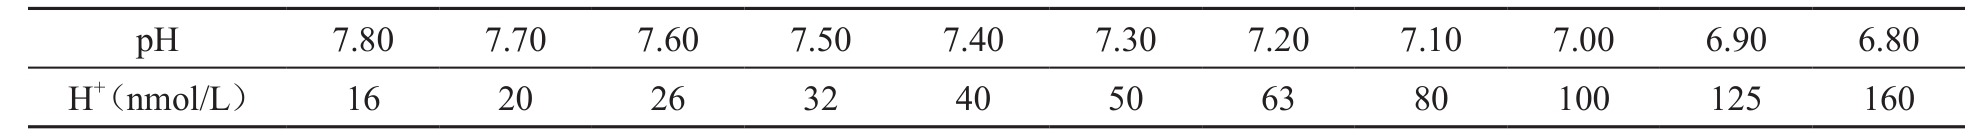
\includegraphics[width=6.60417in,height=0.44792in]{./images/Image00253.jpg}
\end{table}

\subsubsection{缓冲碱(BB)}

缓冲碱(buffer
base,BB)是指全血中具有缓冲作用的阴离子总和。BB以多种形式存在,血浆缓冲碱由血浆中{}
和蛋白质阴离子组成,全血缓冲碱由血浆缓冲碱加上血红蛋白组成,而细胞外液缓冲碱则是由血浆缓冲碱及血红蛋白相当于5g时的缓冲碱组成。在温度37℃、一个标准大气压下,使血样在二氧化碳分压为40mmHg的氧混合气体平衡,并使Hb充分氧合并调整pH至7.40,此时测得的血样BB值为正常缓冲碱,其与实测的缓冲碱的差值为ΔBB。

正常值血浆BB为41~42mmol/L,全血BB为41~48mmol/L,细胞外液BB为43.8mmol/L。正常情况下血浆ΔBB为0,如>
0,证明存在代谢性碱中毒,而<
0则表示存在代谢性酸中毒。由于BB指标不仅受血浆蛋白和Hb的明显影响,而且还受呼吸因素及电解质影响,因此,该指标不能确切反映代谢性酸碱内稳状态。

\subsubsection{碱剩余(BE)}

碱剩余(base
excess,BE)是指在标准条件下(同测定正常缓冲碱标准条件)用酸或碱将1L血液的pH调到7.40所需加入的酸碱量。实际上BE即ΔBB,能表示血浆、全血或细胞外液碱储量增加或减少的量,其为正值时为碱超,如为负值,即碱缺失(base
deficit,BD)。

正常值−3~+
3mmol/L,平均值为0。当BE值正值增大,说明缓冲碱增加,如负值增大,说明缓冲碱减少,因此,BE是反映酸碱平衡失调时代谢性因素的一个客观指标。

\subsubsection{阴离子隙(AG)}

阴离子隙(anion gap,AG)是指血浆中未测定阴离子(undetermined
anion,UA)与未测定阳离子(undetermined cation,UC)的差值,即AG = UA −
UC。由于细胞外液电中性原理,可知Na\textsuperscript{+} + UC =
Cl\textsuperscript{−} +{} + UA,据此可推导出AG的计算公式,即AG = UA − UC
= Na\textsuperscript{+} − Cl\textsuperscript{−} − HCO\textsubscript{3}
\textsuperscript{−} (图\ref{fig68-1})。正常值即140 − 24 − 104 =
12mmol/L,波动范围在12mmol/L ± 2mmol/L。

\begin{figure}[!htbp]
 \centering
 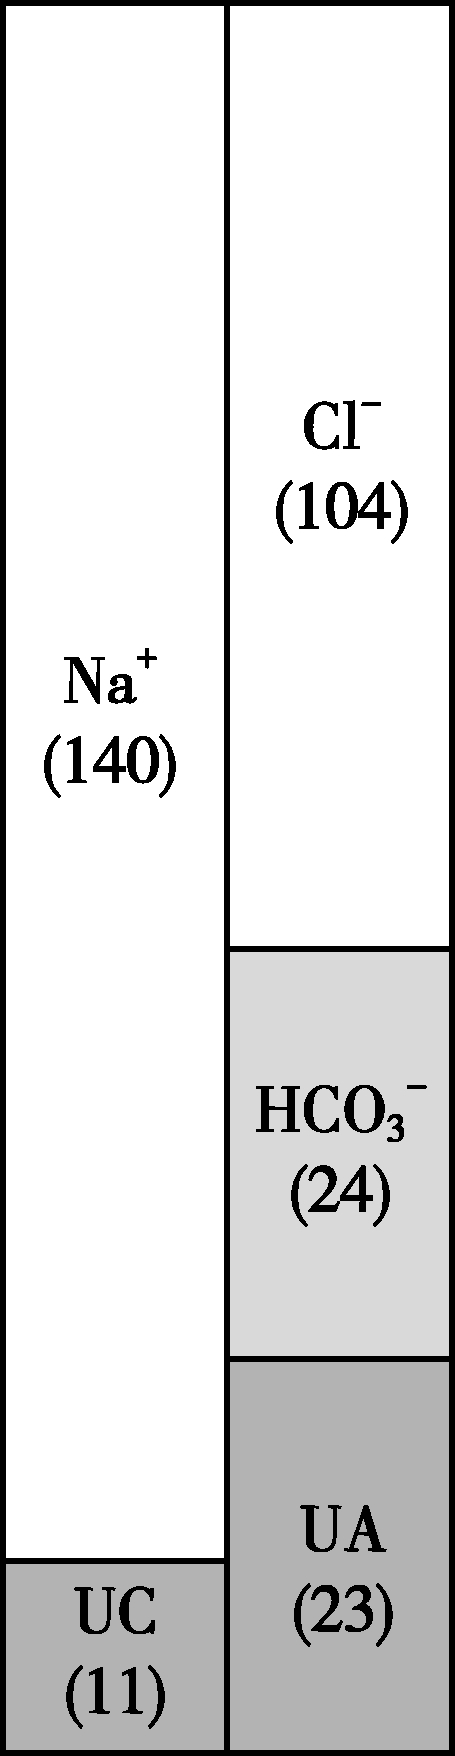
\includegraphics[width=0.75in,height=2.91667in]{./images/Image00256.jpg}
 \captionsetup{justification=centering}
 \caption{血浆阴离子隙图解(mmol/L)}
 \label{fig68-1}
  \end{figure} 

AG可增高也可降低,但增高的临床意义更大:①目前多以AG >
16mmol/L作为判断界限。AG增高表明体内存在过多的UA或固定酸含量增多,即乳酸根、磷酸根及硫酸根等的增多,这些UA在体内堆积,必定要取代{}
,使之下降,从而发生高AG性代谢性酸中毒,因此AG >
16mmol/L,应考虑高AG代谢性酸中毒的存在。②代谢性酸中毒尚可发生于AG正常的情况(详见本章第2节),因此AG增高与否可作为判断代谢性酸中毒类型和原因的依据。③在混合型酸碱平衡紊乱类型判断中,通过计算AG有助于正确的判断(详见本章第7节)。

AG降低在诊断酸碱失衡方面意义不大,仅见于UA减少或UC增多的情况下,如低蛋白血症等。

\subsubsection{潜在{}}

潜在{} (potential bicarbonate)是指排除并存高AG代谢性酸中毒对{}
掩盖作用之后的{}
,用公式表示为潜在
\includegraphics[width=1.47917in,height=0.15625in]{./images/Image00262.jpg}
。其意义可揭示代谢性碱中毒+高AG代谢性酸中毒和三重酸碱紊乱中的代谢性碱中毒存在。若忽视计算潜在HCO\textsubscript{3}
\textsuperscript{−}
和AG,常可延误混合型酸碱紊乱中的代谢性碱中毒的判断。因此下列相关规则应牢记:

高AG代谢性酸中毒:
\includegraphics[width=1.23958in,height=0.13542in]{./images/Image00263.jpg}
,ΔCl\textsuperscript{−} 不变。

高Cl\textsuperscript{−}
性代谢性酸中毒:
\includegraphics[width=1.14583in,height=0.15625in]{./images/Image00264.jpg}
,ΔAG不变。

代谢性碱中毒和呼吸性酸中毒时{}
代偿性↑,符合
\includegraphics[width=1.03125in,height=0.16667in]{./images/Image00266.jpg}
,ΔAG不变。

呼吸性碱中毒时{}
代偿性↓,符合:
\includegraphics[width=0.76042in,height=0.14583in]{./images/Image00268.jpg}
ΔCl\textsuperscript{−} ↑,ΔAG不变。

\protect\hypertarget{text00203.html}{}{}

\section{酸碱平衡失调及机体代偿}

\subsubsection{酸碱平衡调节机制}

正常人的体液保持着一定的pH(动脉血浆pH 7.40 ±
0.05)。动脉血pH降低称为酸血症,反之为碱血症,引起这些改变的紊乱各为酸中毒和碱中毒,而这些改变被定义为“代谢性”(不是因为CO\textsubscript{2}
的增加或减少)或“呼吸性”(由于CO\textsubscript{2}
的原发性增加或减少)。人体代谢过程中由于产酸和产碱使pH经常发生变动,但通过人体的调节作用,pH仅在小范围内变动而保持在7.35~7.45之间。正常机体酸碱平衡的调节机制包括:

\paragraph{体液缓冲系统}

对酸碱失衡能作出最直接和迅速的反应,防止H\textsuperscript{+}
急剧改变,是调节酸碱平衡的首道防线。细胞外液和细胞内液中的弱酸与其共轭碱组成缓冲对,其中HCO\textsubscript{3}
\textsuperscript{−} /H\textsubscript{2} CO\textsubscript{3}
是最重要的一对缓冲物质,两者比值只要保持在20∶1,则血浆的pH仍能保持为7.40。

\paragraph{呼吸调节}

肺通过呼出CO\textsubscript{2}
的多少来调节血液中的呼吸性成分PCO\textsubscript{2}
,即调节血液中的H\textsubscript{2} CO\textsubscript{3}
以维持酸碱平衡,在酸碱失衡时可以发挥呼吸代偿作用,一般在10~30分钟发挥调节作用。当血液H\textsubscript{2}
CO\textsubscript{3}
含量增加、pH下降或低氧血症时,可通过刺激延髓呼吸中枢或外周化学感受器,使呼吸加深加快促使CO\textsubscript{2}
排出增加;反之血液pH增高可减弱对呼吸中枢及化学感受器的刺激,呼吸变得浅慢,肺呼出CO\textsubscript{2}
减少,使H\textsubscript{2} CO\textsubscript{3} 含量增加。

\paragraph{肾脏调节}

是最主要的酸碱平衡调节系统。机体不断产生酸性物质,但肾脏可通过分泌H\textsuperscript{+}
和重吸收{} 以不断补充血液中的{}
,即肾脏通过“排酸保碱”发挥酸碱平衡的调节作用。开始调节最慢,多在数小时以后,但作用最强时间最长,几乎是非挥发性酸和碱性物质排出的唯一途径。调节机制包括:①H\textsuperscript{+}
-Na\textsuperscript{+} 交换;②尿液酸化而排出H\textsuperscript{+}
;③分泌NH\textsubscript{3} 与H\textsuperscript{+} 结合成{} 排出;④{}
的重吸收(图\ref{fig68-2})。

\begin{figure}[!htbp]
 \centering
 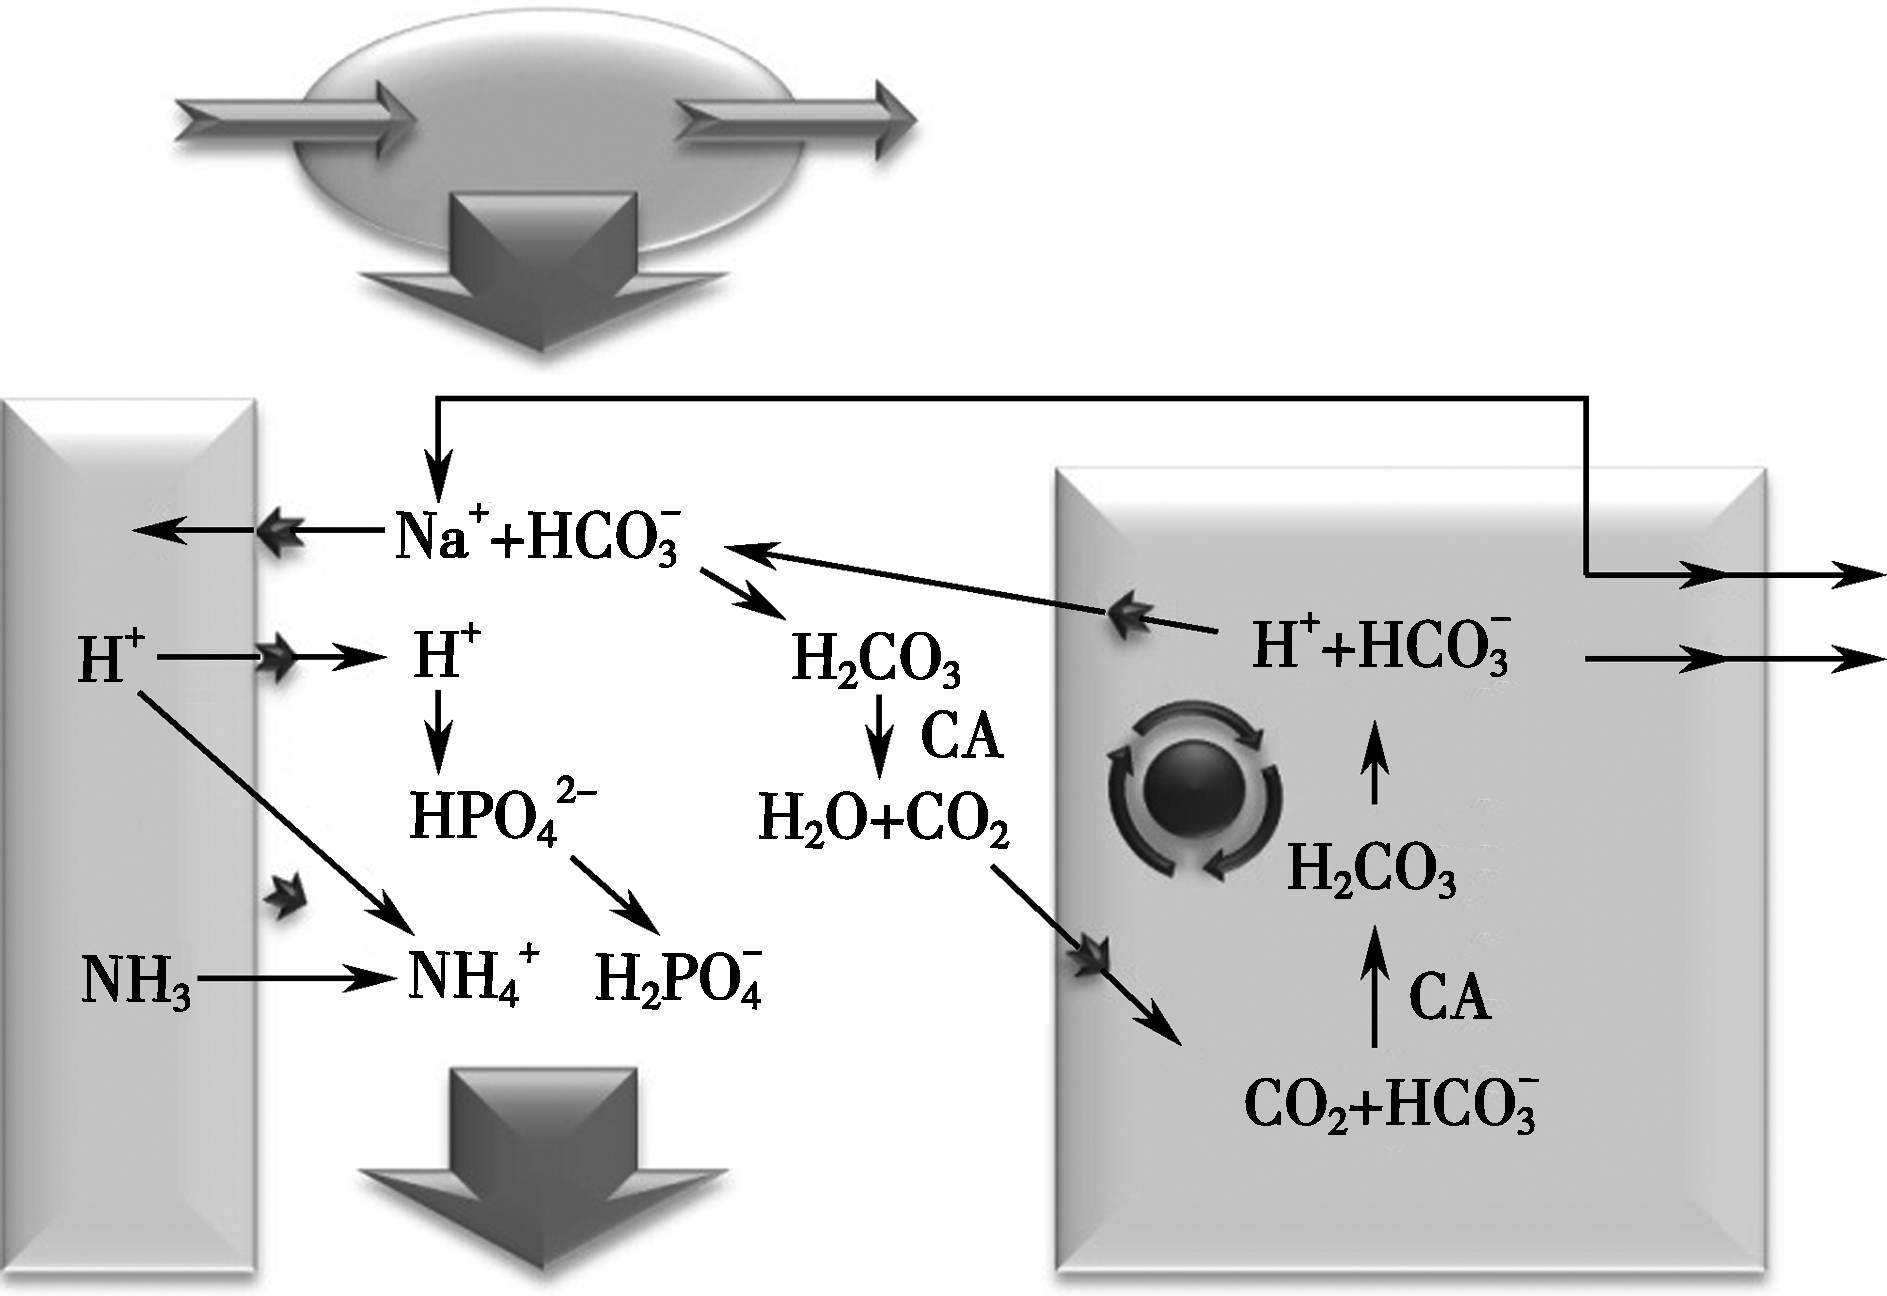
\includegraphics[width=3.13542in,height=2.15625in]{./images/Image00273.jpg}
 \captionsetup{justification=centering}
 \caption{肾脏对酸碱平衡的调节}
 \label{fig68-2}
  \end{figure} 

除以上三种主要调节机制以外
,尚有机体组织细胞的调节作用,组织细胞可通过细胞内外的离子交换和细胞内缓冲系统发挥酸碱平衡的调节作用。

上述各种酸碱平衡调节机制目的是维持体液的pH相对稳定,或在发生酸碱平衡紊乱时发挥代偿作用,但当机体产生酸或碱超过了体内酸碱平衡的代偿能力时,则发生酸或碱中毒。

\subsubsection{酸碱失衡及其代偿反应}

\paragraph{酸碱失衡的临床类型}

当酸碱失衡是因原发性PaCO\textsubscript{2} 或{}
改变所致时,就发生原发性酸碱失衡,或称单纯型酸碱失衡。单纯型酸碱失衡的每一种又可根据pH是否在正常范围分为代偿性与失代偿性两类,还可根据病程和代偿程度分为代偿不足、部分代偿、充分代偿、完全代偿等几种情况。另外,还有两种或两种以上的原发性酸碱失衡同时存在的情况,称为混合型酸碱失衡。但目前认为不存在“呼酸合并呼碱”的情况,除此之外各种组合的混合性酸碱失调都是可能的。如表\ref{tab68-2}。

\begin{table}[htbp]
\centering
\caption{酸碱失衡类型}
\label{tab68-2}
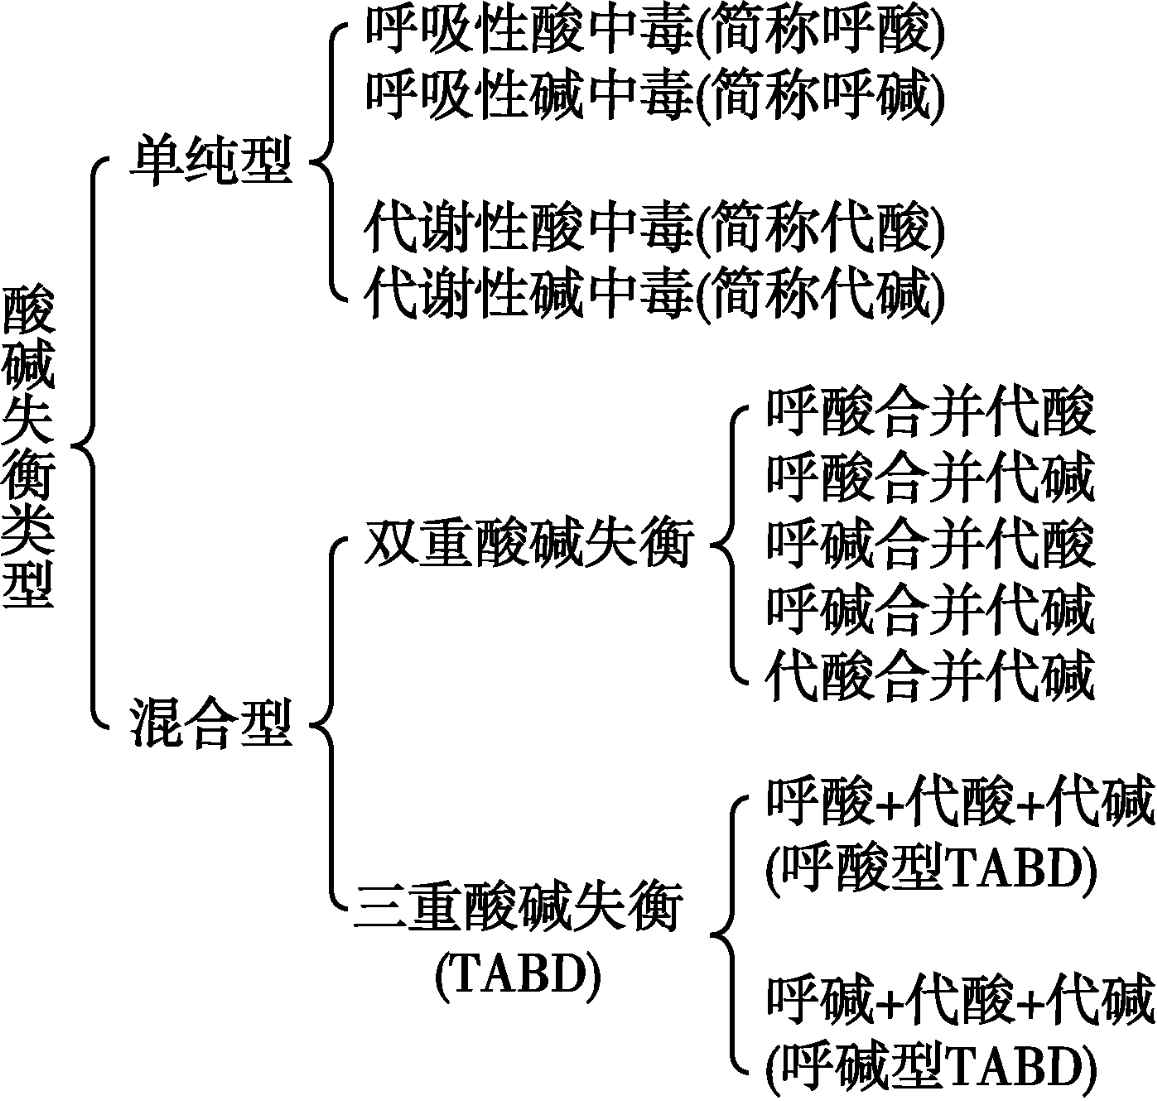
\includegraphics[width=2.32292in,height=2.20833in]{./images/Image00275.jpg}
\end{table}

\paragraph{酸碱失衡代偿反应}

发生酸碱失衡时,缓冲系统、肾脏或呼吸代偿机制发挥作用,通过改变PaCO和{}
,

\textsubscript{2}
力图使其比值维持在适当的比例,使pH回复或趋于正常。代偿反应造成的改变与原发因素的改变呈同一方向,如表\ref{tab68-3}。应注意到肾脏与呼吸的代偿在急性和慢性情况下并不一样,而且代偿改变是有一定限度的。利用代偿预计值方程可以计算代偿反应的预计值高、低限(表\ref{tab68-4}),其用于判断混合型酸碱失衡简便实用且可靠。

\begin{table}[htbp]
\centering
\caption{酸碱失衡的代偿反应}
\label{tab68-3}
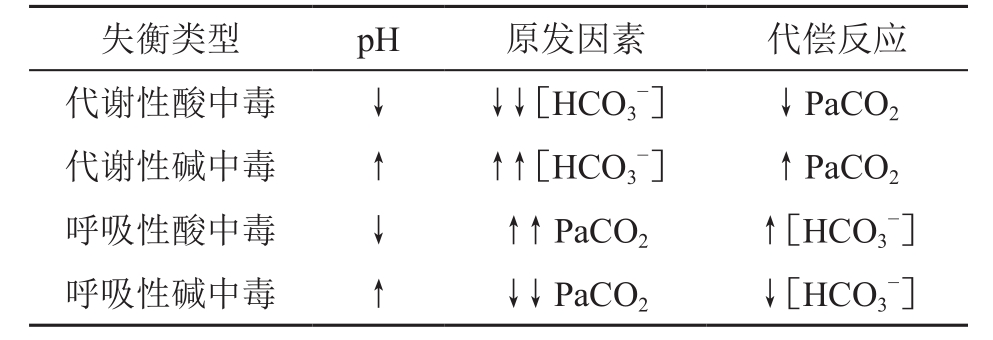
\includegraphics[width=3.30208in,height=1.125in]{./images/Image00277.jpg}
\end{table}

\protect\hypertarget{text00204.html}{}{}

\section{代谢性酸中毒}

代谢性酸中毒(metabolic acidosis,代酸)是由于体内NaHCO\textsubscript{3}
丢失过多或固定酸增多,使{} 消耗过多,导致pH下降,即代谢性酸中毒是血浆{}
含量的原发性减少。

\subsection{病因与发病机制}

\subsubsection{病因}

\begin{table}[htbp]
\centering
\caption{酸碱失衡代偿值预计公式}
\label{tab68-4}
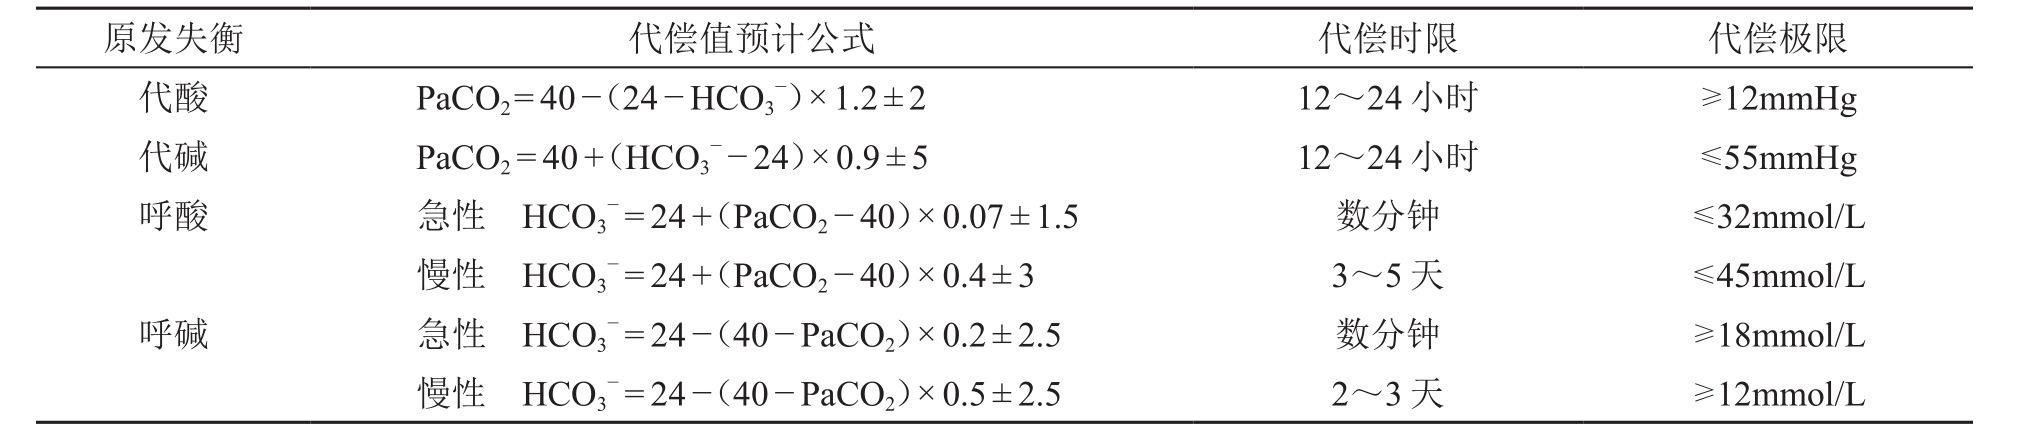
\includegraphics[width=6.72917in,height=1.4375in]{./images/Image00280.jpg}
\end{table}

根据阴离子隙(AG)增高与否,可将代谢性酸中毒分为两类(图\ref{fig68-3}),①高AG代谢性酸中毒,由于血液中大量固定酸的堆积,未测定的阴离子取代血浆{}
,使{} 含量减少,而Cl\textsuperscript{−}
含量不变,因此又称为血氯正常型代谢性酸中毒;②正常AG代谢性酸中毒,由于血浆{}
原发性丢失过多或血Cl\textsuperscript{−} 含量的增加导致肾脏排泄{}
增加,使得AG维持于正常水平,又称为高氯型代谢性酸中毒。两类代谢性酸中毒的常见临床病因见表\ref{tab68-5}。

\begin{figure}[!htbp]
 \centering
 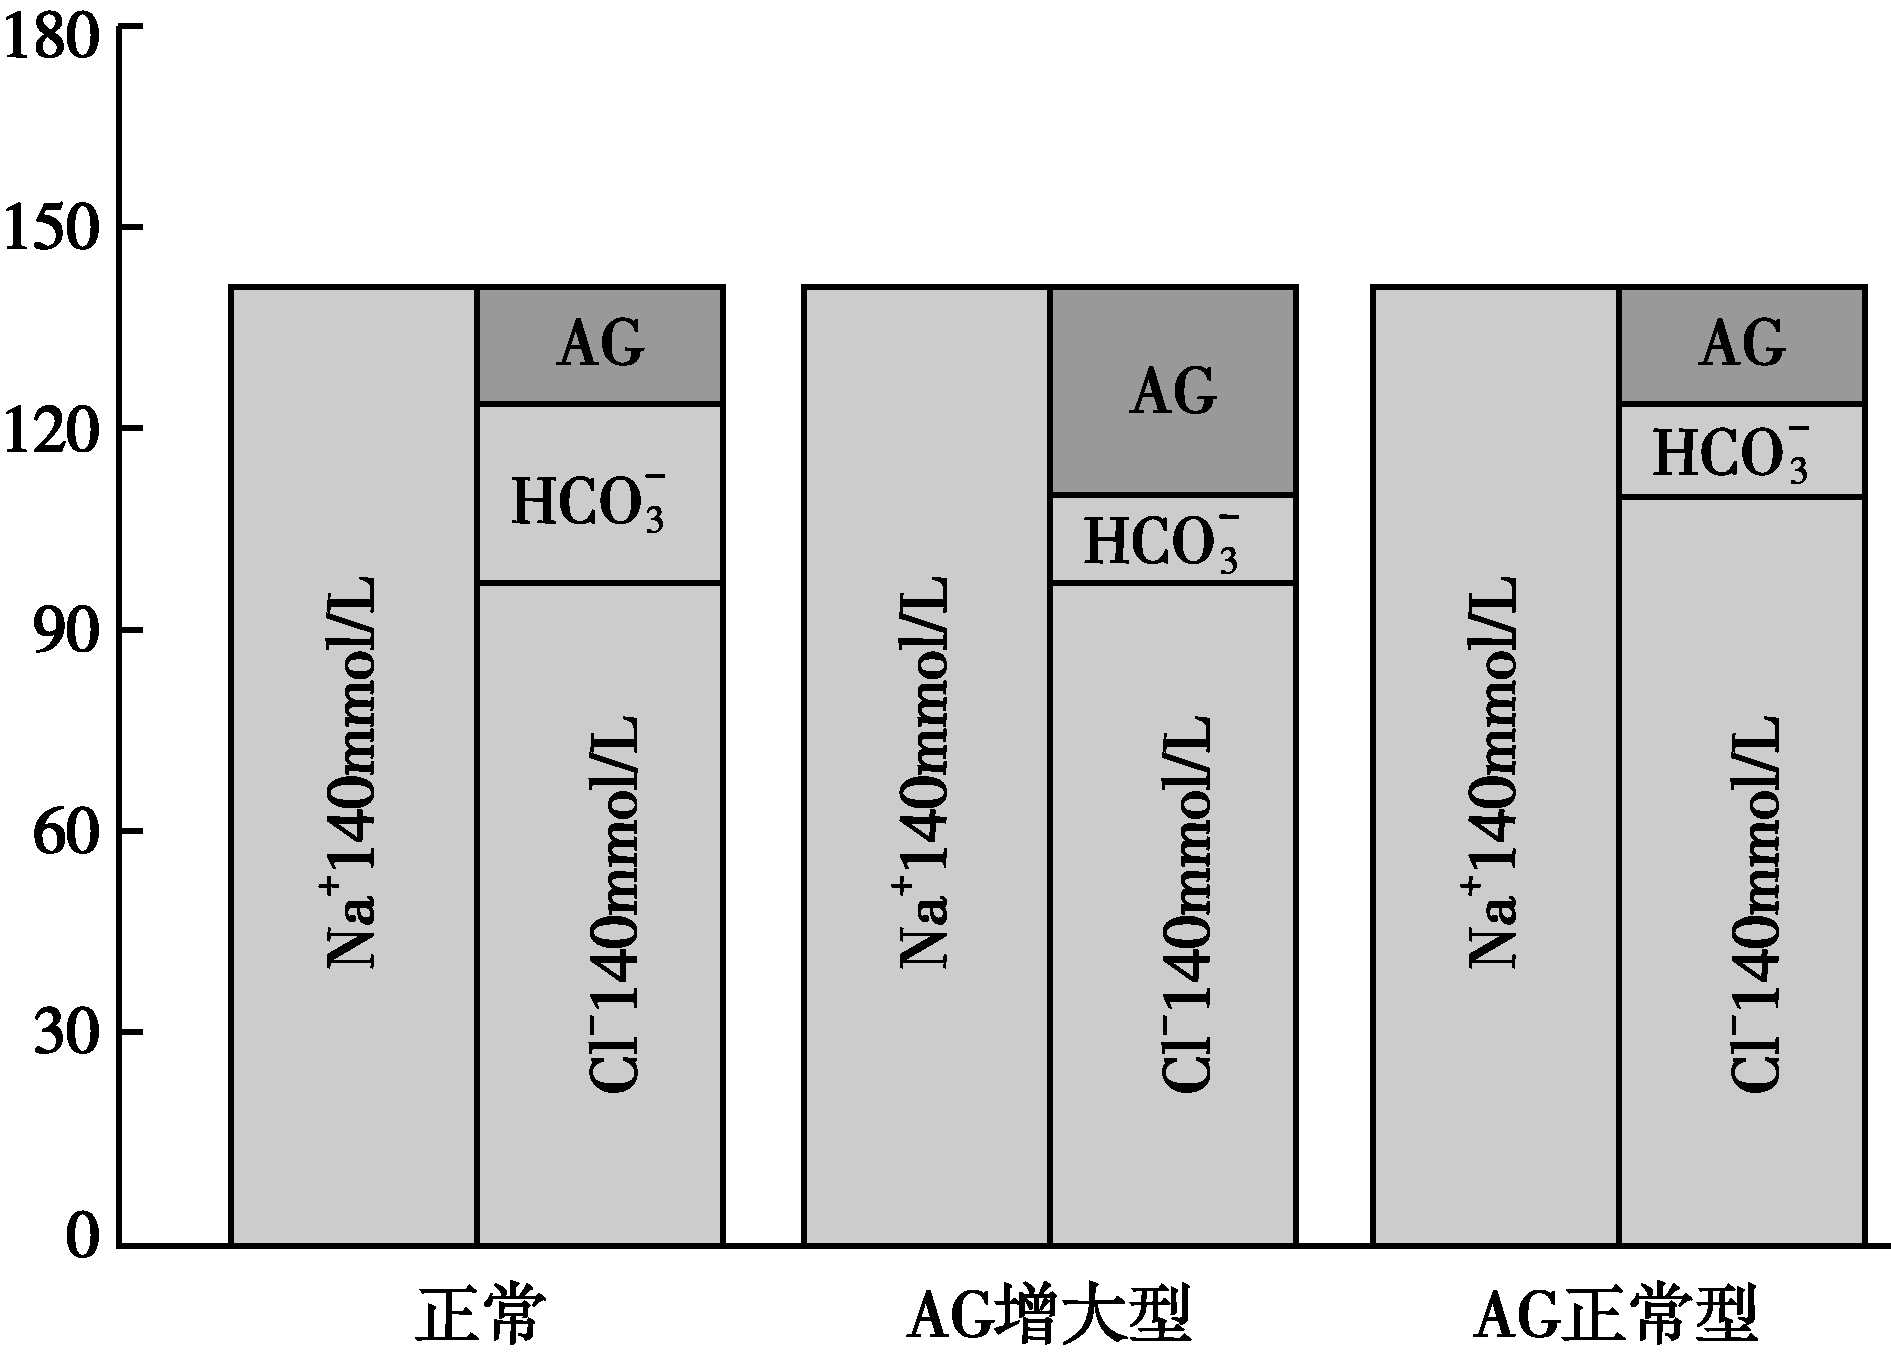
\includegraphics[width=3.11458in,height=2.22917in]{./images/Image00285.jpg}
 \captionsetup{justification=centering}
 \caption{代谢性酸中毒的分类}
 \label{fig68-3}
  \end{figure} 

\begin{table}[htbp]
\centering
\caption{代谢性酸中毒常见病因}
\label{tab68-5}
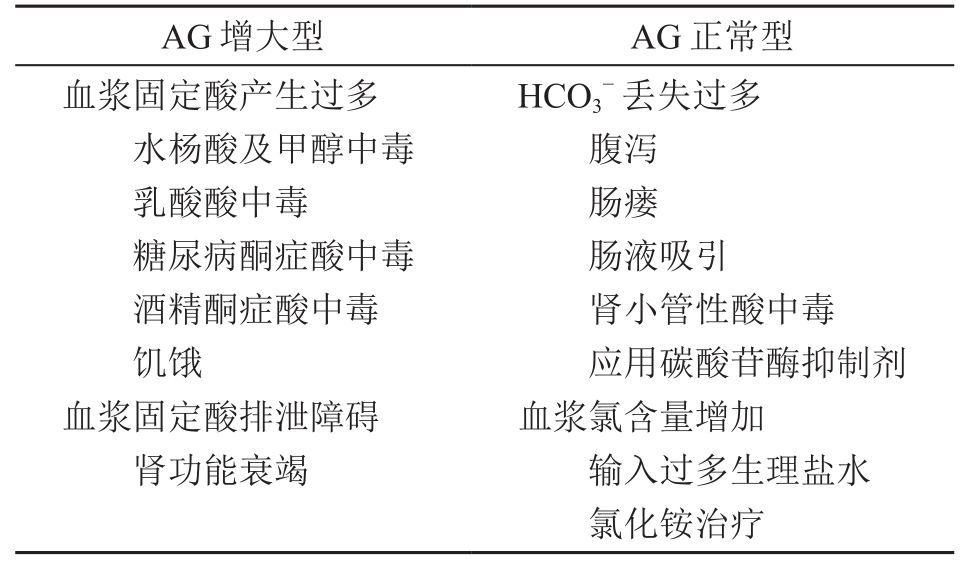
\includegraphics[width=3.22917in,height=1.89583in]{./images/Image00286.jpg}
\end{table}

\subsubsection{代谢性酸中毒的机体反应}

各种原因引起代谢性酸中毒发生后,机体即启动酸碱平衡的各项调节机制发挥代偿反应,主要包括:①血浆缓冲对{}
/H\textsubscript{2} CO\textsubscript{3}
消耗
\includegraphics[width=1.09375in,height=0.14583in]{./images/Image00288.jpg}
,即为失代偿性代谢性酸中毒,pH < 7.35。

代谢性酸中毒的病理生理和临床表现主要包括:①呼吸加深加快,称为Kussmaul呼吸,这是代谢性酸中毒的重要临床表现,少部分患者可因在恢复过程中呼吸加深加快时间过长而发生呼吸性碱中毒;②中枢神经系统可表现为头昏、乏力、嗜睡甚至昏迷,其发生机制在于pH下降促使谷氨酸脱羧酶活性增高,从而在中枢神经系统谷氨酸在该酶作用下更多地转化为γ-氨基丁酸,而γ-氨基丁酸对中枢具有抑制作用;③心血管系统可因pH下降导致心肌代谢障碍、心肌收缩力下降、血管扩张等而表现为不同程度的低血压、心力衰竭等,严重的代谢性酸中毒可导致休克甚至死亡。

\subsection{诊断}

代谢性酸中毒的诊断依据包括:

1.详细了解病史及病情变化、从中找出引起代谢性酸中毒的原因是诊断的最有力依据。

2.临床表现具有非特异性,仅反映代谢性酸中毒的严重程度和代偿情况。

3.辅助检查中动脉血气分析结果重要 ,原发变化是{}
、BE、SB、TCO\textsubscript{2}
减少,血液pH下降,代偿变化是PaCO\textsubscript{2}
下降,血液pH可正常(完全代偿)或降低(代偿不全)。

4.诊断中需注意是否发生混合型酸碱失衡 ,可通过计算PaCO\textsubscript{2}
的代偿预计值来判断。凡实测PaCO\textsubscript{2}
落在预计代偿值范围内,可诊断为代谢性酸中毒;凡实测PaCO\textsubscript{2}
>预计代偿值,可诊断为代谢性酸中毒合并呼吸性酸中毒;凡实测PaCO\textsubscript{2}
<预计代偿值,可诊断为代谢性酸中毒合并呼吸性碱中毒。

\subsection{治疗}

1.病因治疗是根本
应积极去除引起代谢性酸中毒的原因,轻症者经病因治疗后往往能自行恢复,不需特殊处理。

2.严重者应选用碱性药物纠正 应用碱性药物纠正的适应证包括pH <
7.20~7.25,或HCO\textsubscript{3} \textsuperscript{−} <
10~15mmol/L;临床可选用的碱性药物包括:①5\%碳酸氢钠溶液,其纠正酸中毒作用迅速、确切,是较为理想的碱性药物;②11.2\%乳酸钠溶液,其在体内需经肝脏转化为碳酸氢钠而发挥作用,故作用慢,在组织缺氧或肝功能不良等情况下,特别是乳酸酸中毒时不宜应用;③三羟甲基氨基甲烷(THAM),对细胞内外的酸中毒均有纠正作用,在呼吸性酸中毒和代谢性酸中毒时均可使用,但其溶液具有高度碱性(pH
=
10),静滴时应注意不能漏到血管外,以免引起血栓性静脉炎,而且此药大剂量快速静脉给药可抑制呼吸中枢并引起低血压、低血钙等。因此,目前临床上普遍采用的碱性药物是5\%碳酸氢钠溶液,可根据预期{}
浓度,采用公式估算5\%碳酸氢钠溶液的用量,即5\%碳酸氢钠溶液(ml)=(预期{}
− 测得{} )×体重(kg)×
0.5(公式中0.5即0.3/0.6,因细胞外液以系数0.3计算,而5\%碳酸氢钠溶液1ml相当于0.6mmol)。应注意碱性药物不宜补给过多,开始应给予计算量的一半,以后根据监测结果适当补给。

3.如伴有体液电解质代谢失调,应先予以纠正。

\protect\hypertarget{text00205.html}{}{}

\section{呼吸性酸中毒}

呼吸性酸中毒(respiratory acidosis,呼酸)是血浆H\textsubscript{2}
CO\textsubscript{3} 含量的原发性增多,使pH下降。

\subsection{病因与发病机制}

\subsubsection{病因}

临床常见病因包括:①CO\textsubscript{2}
呼出障碍:从呼吸中枢、神经、肌肉到胸廓、气道和肺的各种疾患均可致肺通气不足,致CO\textsubscript{2}
潴留,造成呼吸性酸中毒;②CO\textsubscript{2}
吸入过多:常见于麻醉机的钠石灰效能减低(钠石灰可吸收患者呼出的CO\textsubscript{2}
),使CO\textsubscript{2} 潴留于患者体内而造成呼吸性酸中毒。

\subsubsection{呼吸性酸中毒的机体反应}

呼吸性酸中毒发生后体内缓冲系统和肾脏的调节作用充分发挥其功能,肾脏加强H\textsuperscript{+}
-Na\textsuperscript{+} 的交换,使Na\textsuperscript{+} 和{}
重吸收增加,体内NaHCO\textsubscript{3}
代偿性增多,同时排酸增加。但在急性呼吸性酸中毒时机体主要通过血液、血红蛋白系统和组织缓冲系统的缓冲作用,肾脏几乎不参与代偿,{}
代偿性增加也很有限。在呼吸性酸中毒的发展过程中,细胞内外的离子分布也发生改变,Na\textsuperscript{+}
、K\textsuperscript{+} 从细胞内向细胞外转移,而H\textsuperscript{+}
进入细胞内,H\textsuperscript{+}
的转移有助于提高细胞外液pH,但K\textsuperscript{+}
向细胞外转移使血清K\textsuperscript{+}
浓度升高却对机体有害。急性呼吸性酸中毒时,血清{[}K\textsuperscript{+}
{]}迅速升高,极易引起患者室颤而死亡。

呼吸性酸中毒对中枢神经、循环系统等的影响与代谢性酸中毒相同,但较代谢性酸中毒更易导致中枢神经系统功能障碍。因为正常情况下呼吸中枢对动脉血CO\textsubscript{2}
含量很敏感,但当血CO\textsubscript{2}
过度聚积,浓度达到9\%时,呼吸中枢就失去对CO\textsubscript{2}
的敏感性,如CO\textsubscript{2}
浓度继续升高,将导致呼吸中枢麻痹,发生昏迷甚至死亡。

\subsection{诊断}

临床上常可根据呼吸功能受影响的病史和体征,结合动脉血气分析相关指标,作出初步诊断。动脉血气分析结果中原发变化是PCO\textsubscript{2}
上升,使血液pH下降,代偿变化是{} 、BE、SB、TCO\textsubscript{2}
等增加,pH可能回到正常。诊断时需考虑是否合并其他类型酸碱失衡,可通过计算{}
的代偿预计值来判断,如实测{[}{}
{]}落在代偿预测值范围内者,可诊断急性或慢性呼酸;实测{}
>代偿预测值范围上限时,可诊断为急性或慢性呼酸合并代碱;当实测{}
<代偿预测值范围下限时,可诊断为急性或慢性呼酸合并代酸。

\subsection{治疗}

1.病因治疗是根本,改善通气是关键。应针对病因解除呼吸道梗阻,紧急时可进行气管插管或气管切开,实施机械通气治疗。

2.呼吸中枢受抑制,可根据病情及时人工呼吸或使用呼吸兴奋剂。

3.原则上不宜用碱性药物 ,只有在pH <
7.20,出现危及生命的酸血症而同时具备机械通气条件时方予补碱。补碱可用THAM,也可用5\%碳酸氢钠溶液。

4.伴高钾血症时,按高钾血症处理。

治疗过程中应注意两点,一是不能单纯给氧,否则会因血氧浓度过高导致呼吸中枢感受器对缺氧刺激反射消失,从而进一步抑制呼吸;二是纠正酸中毒时考虑“宁酸毋碱”原则,以免加重组织缺氧和抑制呼吸。

\protect\hypertarget{text00206.html}{}{}

\section{代谢性碱中毒}

代谢性碱中毒(metabolic
alkalosis,代碱)是指碱性物质在体内积蓄过多或酸性物质的大量丢失,造成血浆{}
浓度原发性升高,使pH上升。

\subsection{病因与发病机制}

\subsubsection{病因}

临床常见代谢性碱中毒的原因包括:①酸性胃液的大量丢失,肠液{}
重吸收增加。正常情况下含有盐酸的胃液进入肠内与肠液中的{}
中和,然后由肠黏膜吸收回血流,这是血液得以保持酸碱平衡的重要条件之一。当大量胃液由于呕吐或胃引流术而大量丧失时,上述生理变化遭到破坏,肠液中的{}
未被盐酸中和即回到血液,故血液中的{}
含量增加而发生碱中毒,pH升高。②治疗溃疡病时碱性药物服用过多。如过多服用小苏打(碳酸氢钠),其在胃中与盐酸中和,使胃酸消失或明显减少,因而肠液中的{}
不能为胃酸中和而直接吸收入血,造成碱中毒。③Cl\textsuperscript{−}
大量丢失。利尿剂的大量应用可造成低氯血症,使得肾近曲小管对{}
和Na\textsuperscript{+}
重吸收增加,造成低氯性碱中毒。④缺钾性碱中毒。低钾血症时细胞内K\textsuperscript{+}
向细胞外转移,细胞外Na\textsuperscript{+} 和H\textsuperscript{+}
向细胞内转移,使得细胞外液中H\textsuperscript{+}
减少,造成细胞外液碱中毒肾小管细胞中的H\textsuperscript{+}
和K\textsuperscript{+} 均与肾小管液中的Na\textsuperscript{+}
进行交换,低钾患者肾小管细胞内K\textsuperscript{+}
减少时,肾排K\textsuperscript{+} 保Na\textsuperscript{+}
能力减弱,排H\textsuperscript{+} 保Na\textsuperscript{+}
加强,使排酸增加,肾重吸收入血NaHCO\textsubscript{3}
增多,导致碱中毒加重。

\subsubsection{代谢性碱中毒的机体反应}

代谢性碱中毒时,pH升高抑制延髓呼吸中枢,患者呼吸变浅变慢,CO\textsubscript{2}
排出减少,血液中H\textsubscript{2} CO\textsubscript{3}
含量升高,使得NaHCO\textsubscript{3} /H\textsubscript{2}
CO\textsubscript{3}
比值接近正常,从而发生代谢性碱中毒。如碱中毒持续存在,将通过肾排出过多{}
以调节体液pH,但由于肾对代谢性碱中毒的调节作用主要由体内K\textsuperscript{+}
、Cl\textsuperscript{−} 水平决定,当低K\textsuperscript{+}
、脱水或低Cl\textsuperscript{−} 血症时,肾仍保持对NaHCO\textsubscript{3}
的重吸收,而不能发挥对碱中毒的代偿作用。

代谢性碱中毒导致的病理生理变化引起相应的临床表现:①呼吸浅慢,系由代谢性碱中毒时的呼吸调节作用导致。②神经肌肉应激性增高,表现为口角抽动,手足搐搦,腱反射亢进等,其原因在于血液偏碱时血中Ca\textsuperscript{2+}
浓度降低。③中枢神经系统功能障碍,如烦躁不安,精神错乱,谵妄等,其发生机制主要是pH升高后γ-氨基丁酸转氨酶活性增强,使得中枢神经细胞内谷氨酸生成增加,而谷氨酸系中枢兴奋性氨基酸。

\subsection{诊断}

强调确定发生代谢性碱中毒的病因对诊断的重要性。除根据临床症状外,还应根据血电解质变化和动脉血气分析结果作出诊断。动脉血气分析结果中原发性变化为{}
、BE、SB、TCO\textsubscript{2}
等增加,血液pH上升;代偿性变化为PaCO\textsubscript{2}
上升(代偿往往不全),肾排出碱性尿(低钾碱时呈酸性尿)。

可通过计算PaCO\textsubscript{2}
的代偿预计值来判断是否合并其他类型酸碱失衡,凡实测PaCO\textsubscript{2}
落在预计值范围内,可诊断为代谢性碱中毒;实测PaCO\textsubscript{2}
>预计代偿值,可诊断为代谢性碱中毒合并呼吸性酸中毒;实测PaCO\textsubscript{2}
<预计代偿值,可诊断为代谢性碱中毒合并呼吸性碱中毒。

\subsection{治疗}

1.以病因治疗为根本。

2.氯敏感性代碱可补充氯化钠 、氯化钾、氯化铵,重症者可补酸。

3.氯不敏感性代碱可补钾 、用保钾类利尿剂、乙酰唑胺等,甚至透析。

4.常用酸性药物有盐酸精氨酸(10g≈HCl
48mmol)、稀盐酸(50~200mmol/L)、氯化铵等。

5.碱血症致抽搐者,可补钙剂。

\protect\hypertarget{text00207.html}{}{}

\section{呼吸性碱中毒}

呼吸性碱中毒(respiratory alkalosis,呼碱)是血浆H\textsubscript{2}
CO\textsubscript{3} 含量的原发性降低,致pH上升。

\subsection{病因与发病机制}

\subsubsection{病因}

呼吸性碱中毒临床少见,可见于下列情况:①各种原因引起的呼吸中枢受刺激或肺部疾患导致过度通气,体内CO\textsubscript{2}
丧失过多,见于癔症发作、颅脑损伤、缺氧及小儿大哭等。②机械通气不当,造成人为过度通气。

\subsubsection{呼吸性碱中毒的机体反应}

呼吸性碱中毒时的代偿反应主要是由于血液CO\textsubscript{2}
减少,CO\textsubscript{2}
弥散入肾小管细胞量减少,造成肾小管泌H\textsuperscript{+}
作用减少,H\textsuperscript{+} -Na\textsuperscript{+} 交换减弱,{}
重吸收减少,导致血浆{} 水平也降低。

发生呼吸性碱中毒时,患者自觉头晕、胸闷,呼吸快浅或短促,但呼吸减慢后CO\textsubscript{2}
排出减少,上述症状可自行缓解。因碱中毒时血Ca\textsuperscript{2+}
减少,患者可出现肌肉震颤、手足搐搦等。碱中毒时尚可使血红蛋白对氧的亲和力增加,导致组织细胞氧利用发生障碍,引起组织缺氧,可表现为眩晕、昏厥、意识障碍等。

\subsection{诊断}

呼吸性碱中毒的诊断主要依据病史和动脉血气分析检测。动脉血气分析结果中原发性变化是PaCO\textsubscript{2}
下降,使血液pH上升;代偿性变化包括{} 、BE、SB、TCO\textsubscript{2}
等下降,pH可能回到正常,Cl\textsuperscript{−} 增高,K\textsuperscript{+}
轻度降低,AG轻度增高。

计算{[}{} {]}的代偿预计值提示,如实测{}
在代偿预测值范围内时,可诊断为急性或慢性呼碱;实测{}
>代偿预测值范围上限时,可诊断为急性或慢性呼碱合并代碱;实测{}
<代偿预测值范围下限时,可诊断为急性或慢性呼吸碱合并代酸。

\subsection{治疗}

1.解除病因,积极处理原发病。

2.对症处理可使用纸袋
、长筒等罩住口鼻,以增加死腔间隙,减少CO\textsubscript{2}
呼出,或采取吸入含5\% CO\textsubscript{2} 的氧气,可改善症状。

3.纠正低钾、高氯血症。

\protect\hypertarget{text00208.html}{}{}

\section{混合型酸碱平衡失调}

一般情况下,机体有代偿机制,使{} /H\textsubscript{2} CO\textsubscript{3}
维持在20/1,但有时仍出现原发性代谢性和原发性呼吸性酸碱失常。两种或三种单纯型酸碱平衡紊乱同时存在时,称为混合型酸碱平衡失调(mixed
acid-base
disorders)。根据同时合并酸碱平衡紊乱的性质,可以分为二重性或双重性酸碱平衡紊乱(double
acid-base disorders)及三重酸碱平衡紊乱(triple acid-base
disorders,TABD)。混合型酸碱失常时,原有代偿反应不复存在。

\subsubsection{代谢性碱中毒合并呼吸性碱中毒}

创伤后常因疼痛、颅脑损伤、低氧血症、脓毒血症、机械过度通气而有呼吸性碱中毒。但同时又因呕吐、胃管引流、大量输血而合并代谢性碱中毒。出现PaCO\textsubscript{2}
下降,{}
升高,两者都使pH升高,当pH超过7.55~7.60时.可能出现心排血量降低、心律失常、脑和冠状血管收缩、血红蛋白氧离曲线左移、心脑缺氧,患者进入高危状态。此型有严重的碱血症,pH明显升高;两型碱中毒合并存在时{}
与PaCO\textsubscript{2}
的变化因相互抵消而变化不如单纯型碱中毒明显;对代碱来说,PaCO\textsubscript{2}
测定值低于代偿预估值;对呼碱来说,{} 测定值大于代偿预估值。

\subsubsection{代谢性碱中毒合并呼吸性酸中毒}

患者的呼吸功能因呼吸道梗阻、肺受压(如胸水、气胸)而有呼吸性酸中毒,而同时又因大量胃肠液的丢失、大量输血等而有代谢性碱中毒,pH虽可在正常范围,实际上是代谢性碱中毒与呼吸性酸中毒同时存在。急慢性呼吸性酸中毒伴有{}
的不适当升高或代谢性碱中毒伴有PaCO\textsubscript{2}
的不适当升高均可诊断为本型。酸碱指标特点为PaCO\textsubscript{2} 升高,{}
升高,pH升高、正常或下降。多见于慢性肺功能不全患者呕吐、利尿或氯缺乏。

\subsubsection{代谢性酸中毒合并呼吸性酸中毒}

在胸部或中枢神经系统疾患的患者,由于呼吸功能障碍而有呼吸性酸中毒。如又有组织灌注不足、缺氧而出现代谢性酸中毒,因此,pH急骤下降。治疗时,除积极改善肺的通气功能,应用机械通气治疗外,还应改善组织灌注,对pH低于7.10~7.15者,要适当抗酸,使pH升至7.20以上,在纠正酸中毒时,要及时补钾,以防血钾大幅度降低。急慢性呼吸性酸中毒伴有不适当的{}
下降或者代谢性酸中毒伴有不适当的PaCO\textsubscript{2}
增加均可诊断为本型。一般原发变化比继发变化显著,多为“矛盾地”出现{}
降低而PaCO\textsubscript{2} 增高,由预估值公式可得出{}
测定值低于预估值而PaCO\textsubscript{2}
测定值大于预估值。患者血浆Cl\textsuperscript{−}
可低、高或正常;AG可增高;血浆K\textsuperscript{+}
多增高,若有低K\textsuperscript{+} 则表示严重K\textsuperscript{+} 缺乏。

\subsubsection{代谢性酸中毒合并呼吸性碱中毒}

中枢神经系统疾患、应用机械通气、多发损伤、疼痛、发热、情绪紧张的患者常有呼吸性碱中毒,但是由于缺氧、缺血引起乳酸性酸中毒,出现呼吸性碱中毒与代谢性酸中毒并存,pH虽改变不明显,而PaCO\textsubscript{2}
和{}
下降均超过正常范围。在治疗同时解决产生呼吸性碱中毒与代谢性酸中毒的病因。代谢性酸中毒伴有PaCO\textsubscript{2}
的不适当下降或呼吸性碱中毒伴有{}
的不适当下降即可判断为此型。应用代偿公式计算预计PaCO\textsubscript{2}
或{}
有助于进行判断。见于水杨酸中毒者、肾功衰竭或糖尿病酮症伴有高热呼吸过度者或严重肝病或败血症者。此型pH可高可低或正常;{}
与PCO\textsubscript{2}
都降低,明显低于单一型的预估值;血浆Cl\textsuperscript{−}
常增高;AG可轻度或中度升高;BE负值加大。

\subsubsection{代谢性酸中毒合并代谢性碱中毒}

见于肾功能衰竭或糖尿病酮症酸中毒或乳酸中毒患者发生呕吐、胃液引流时。血液生化特征:pH变化不明显;{}
与PCO\textsubscript{2}
变化相反。高AG代谢性酸中毒合并代谢性碱中毒的诊断:单纯型高AG代谢性酸中毒时,AG的升高与{}
的下降呈1∶1,若发现AG升高并没有使{}
相应下降甚至升高,即可诊断为高AG代谢性酸中毒合并代碱。同理,单纯型代谢性碱中毒若并发乳酸酸中毒,则{}
下降必然有相应的AG增加,当AG增加,而{}
未相应下降时,则肯定有混合性的代谢性酸中毒和代谢性碱中毒存在。正常AG代谢性酸中毒合并代谢性碱中毒的诊断:单纯型代谢性碱中毒是低Cl\textsuperscript{−}
和高{} ,而正常AG代谢性酸中毒是高Cl\textsuperscript{−} 和低{}
,所以当两种紊乱同时并存且程度相当时,作用正好相互抵消,表现出大致正常的酸碱、血气和电解质值,必须依靠病史和病情分析才能对该型作出诊断。

\subsubsection{三重性酸碱平衡紊乱}

一种呼吸性酸碱紊乱(呼吸性酸中毒或呼吸性碱中毒)合并代谢性酸中毒加代谢性碱中毒称为三重性酸碱紊乱(TABD)。呼吸性碱中毒+代谢性碱中毒+代谢性酸中毒(呼碱型TABD)可见于在呼吸性碱中毒合并代谢性碱中毒的基础上,再合并高AG代谢性酸中毒,也可见于在呼吸性碱中毒合并高AG代谢性酸中毒的基础上,由于补碱过多再合并代谢性碱中毒;本型紊乱酸碱指标特点为:AG升高,PaCO\textsubscript{2}
下降以及{}
变化与AG升高不成对等比例,pH取决于三种紊乱的相对严重程度。呼吸性酸中毒+代谢性酸中毒+代谢性碱中毒(呼酸型TABD)多见于较为严重的肺心病呼吸衰竭时,其酸碱指标特点为:AG升高,{}
变化与AG升高不成对等比例,而pH变化不定。

\protect\hypertarget{text00209.html}{}{}

\section{酸碱平衡失调的判断方法}

酸碱平衡失调是临床的基本问题和共性问题之一,对其正确及时的判断常常是治疗成败的关键。酸碱平衡失调的判断能否对治疗起指导作用,关键又在于判断是否正确。临床上有很多方法用于判断酸碱平衡失调的类型,无论哪种判断方法,首先必须掌握必要的判断依据。

\subsubsection{酸碱平衡失调的判断依据}

\paragraph{病史}

提供酸碱失衡的病因线索,估计失衡的代偿时间。

\paragraph{临床表现}

缺乏特异性,可核实血气判断,估计失衡程度。

\paragraph{血气分析和血清电解质测定}

是主要依据。血气分析中的多项指标均与酸碱平衡有关,但判断酸碱失衡必备的主要指标有pH、PaCO\textsubscript{2}
、{} 三项,其余指标均作参考。

\paragraph{阴离子隙(AG)}

AG是一项近年来很受重视的酸碱指标,AG增高常反映有机酸中毒或高AG代酸及其程度,AG是判断混合代谢型酸碱失衡的重要指标。

\paragraph{尿 pH和尿电解质测定}

对分析酸碱失衡原因有帮助。

\paragraph{其他}

血细胞比容、血浆蛋白、血浆渗透压等有时也可参考。

\subsubsection{酸碱平衡失调类型的判断}

\hypertarget{text00209.htmlux5cux23CHP6-5-8-2-1}{}
(一) 一般判断方法

1.分清原发和代偿变化
①了解病史,考虑该疾病发生酸碱紊乱是什么性质;②估计酸碱失衡持续时间,是急性还是慢性;③患者用药、给氧与电解质情况;④肾功能、肺功能等检查结果。

2.分析主要指标(pH、PaCO\textsubscript{2} 、BE),初步判断紊乱类型:

(1) 由pH进行判断:当pH < 7.35,即可诊断酸血症;pH >
7.45,即诊断碱血症;若pH正常,则表示该血液的酸碱状态正常,但不能排除可能存在的酸中毒或碱中毒。

(2) 由PaCO\textsubscript{2} 和{} 进行判断:①PaCO\textsubscript{2} <
35mmHg,应考虑呼吸性碱中毒;PaCO\textsubscript{2} >
45mmHg,应考虑呼吸性酸中毒;
\includegraphics[width=0.5in,height=0.11458in]{./images/Image00340.jpg}
27mmol/L,应考虑代谢性碱中毒;AG >
16mmol/L,应考虑代谢性酸中毒。②根据PaCO\textsubscript{2}
和HCO\textsubscript{3} \textsuperscript{−}
测定数值,查酸碱诊断检索表(表\ref{tab68-6})进行酸碱紊乱类型的初步判断。③若临床症状不明显而pH异常,则可从PaCO(\textsubscript{2}
mmHg)与{} (mmol/L)变化程度进行区别,方法如下:

pH < 7.40,{} × PaCO\textsubscript{2} >
1000,应考虑呼酸(因PaCO\textsubscript{2} ↑↑↑及{} ↑)。

pH < 7.40,{} × PaCO\textsubscript{2} <
1000,应考虑代酸(因PaCO\textsubscript{2} ↓及{} ↓↓↓)。

pH > 7.40,{} × PaCO\textsubscript{2} <
1000,应考虑呼碱(因PaCO\textsubscript{2} ↓↓↓及{} ↓)。

pH > 7.40,{} × PaCO\textsubscript{2} >
1000,应考虑代碱(因PaCO\textsubscript{2} ↑及{} ↑↑↑)。

\begin{table}[htbp]
\centering
\caption{酸碱诊断检索表}
\label{tab68-6}
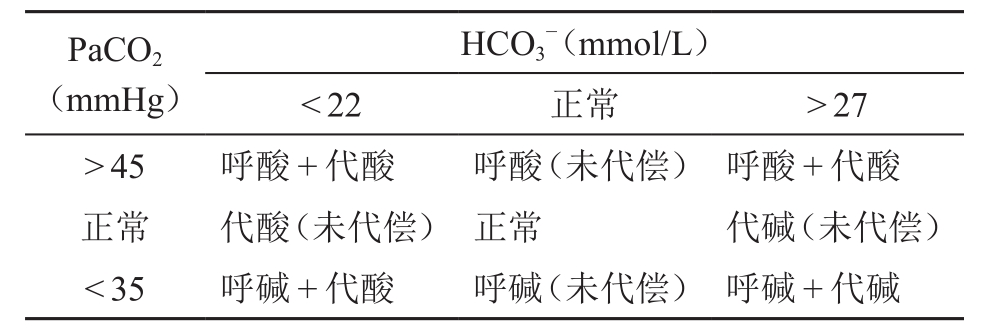
\includegraphics[width=3.26042in,height=1.09375in]{./images/Image00350.jpg}
\end{table}

3.鉴别单纯型和混合型酸碱平衡失调
①初步分析,根据病因和病情发展判断原发性酸碱平衡失调类型。②根据公式计算PaCO\textsubscript{2}
或{}
的代偿预计值,根据实测值与代偿预计值范围的关系判断是否存在混合型酸碱平衡紊乱。③掌握代偿时间有助于分析酸碱平衡失调是急性还是慢性,是部分代偿还是最大代偿,是单纯型还是混合型紊乱。

4.动态观察和综合分析。

\hypertarget{text00209.htmlux5cux23CHP6-5-8-2-2}{}
(二) 四步判断法

此法是一种筛选判断法
,有较高准确性和可靠性,具有明确的程序和数据可循,简便实用,可作为临床常规判断应用。以下介绍本法的具体步骤及其设计的理论依据。

第一步:根据PaCO\textsubscript{2} 与{}
的实测值与正常值的比较确定属于图\ref{fig68-4}\footnote{注:△△表示代偿预计值高限;△表示代偿预计值低限;N表示代偿预计值范围}内(A)、(B)、(C)、(D)中的哪一组。

第二步:如果为(A)或(C)组,则根据PaCO\textsubscript{2} ×
0.6与HCO\textsubscript{3} \textsuperscript{−}
的大小比较或pH的高低,确定属于表中(A)(1)、(2)、(3)中的哪一组,然后按该组右侧提示的失衡类型作出两种可能的判断;结合病史、临床表现和相关化验结果确定是哪一种;应牢记病史中病因或病情变化对于判断原发性酸碱平衡紊乱类型的重要性,只有从病因或者病情发展中才能明确原发性酸碱平衡失调的性质是代谢性抑或呼吸性。例如(A)(3)组提示有“代谢性碱中毒”或“呼吸性酸中毒合并代谢性碱中毒”两种可能性,这对一例肺部急性感染5天的肺心病患者来说,理应判断为后者,而对一原先体健,因严重呕吐入院的患者来说则应判断为前者;需要指出的是,如果病情中同时存在两种病因时,则应以首先出现的病因为依据来确定诊断。

如果属于(B)或(D)组,则可立即得出两种可能的判断,然后根据病史等确定最后诊断。

第三步:计算代偿预计值。如果第二步确定是单纯型酸碱平衡失调,则根据相应公式计算PaCO\textsubscript{2}
或{}
的代偿预计值高低限。如实测值在高低限范围内,则应判断为代偿性单纯型酸碱平衡失调;如果高于高限,或低于低限,则可根据表中右侧括号内的提示,判断为失代偿性单纯型酸碱平衡失调或混合型酸碱平衡失调,并根据病史等确定符合病情的判断。

第四步:计算AG值。如AG <
14mmol/L,则前三步判断结果就是最后诊断类型;如AG >
16mmol/L,而且病史、临床表现及有关化验结果亦提示代谢性酸中毒的存在,则可判断为代谢性酸中毒,然后将前三步判断结果结合AG的增高按下列步骤确定最后诊断:

1.如前三步判断是呼吸性酸中毒
+代谢性碱中毒或呼吸性碱中毒+代谢性碱中毒,而AG >
16mmol/L提示存在代谢性酸中毒,则最后判断是呼酸型TABD或呼碱型TABD。

2.如前三步判断是呼吸性酸中毒
、呼吸性碱中毒、呼吸性酸中毒+代谢性酸中毒或呼吸性碱中毒+代谢性酸中毒,由于AG
>
16mmol/L,那么首先均分别判断是呼吸性酸中毒+代谢性酸中毒或呼吸性碱中毒+代谢性酸中毒,而是否存在代谢性碱中毒,需要进一步判断:

\begin{figure}[!htbp]
 \centering
 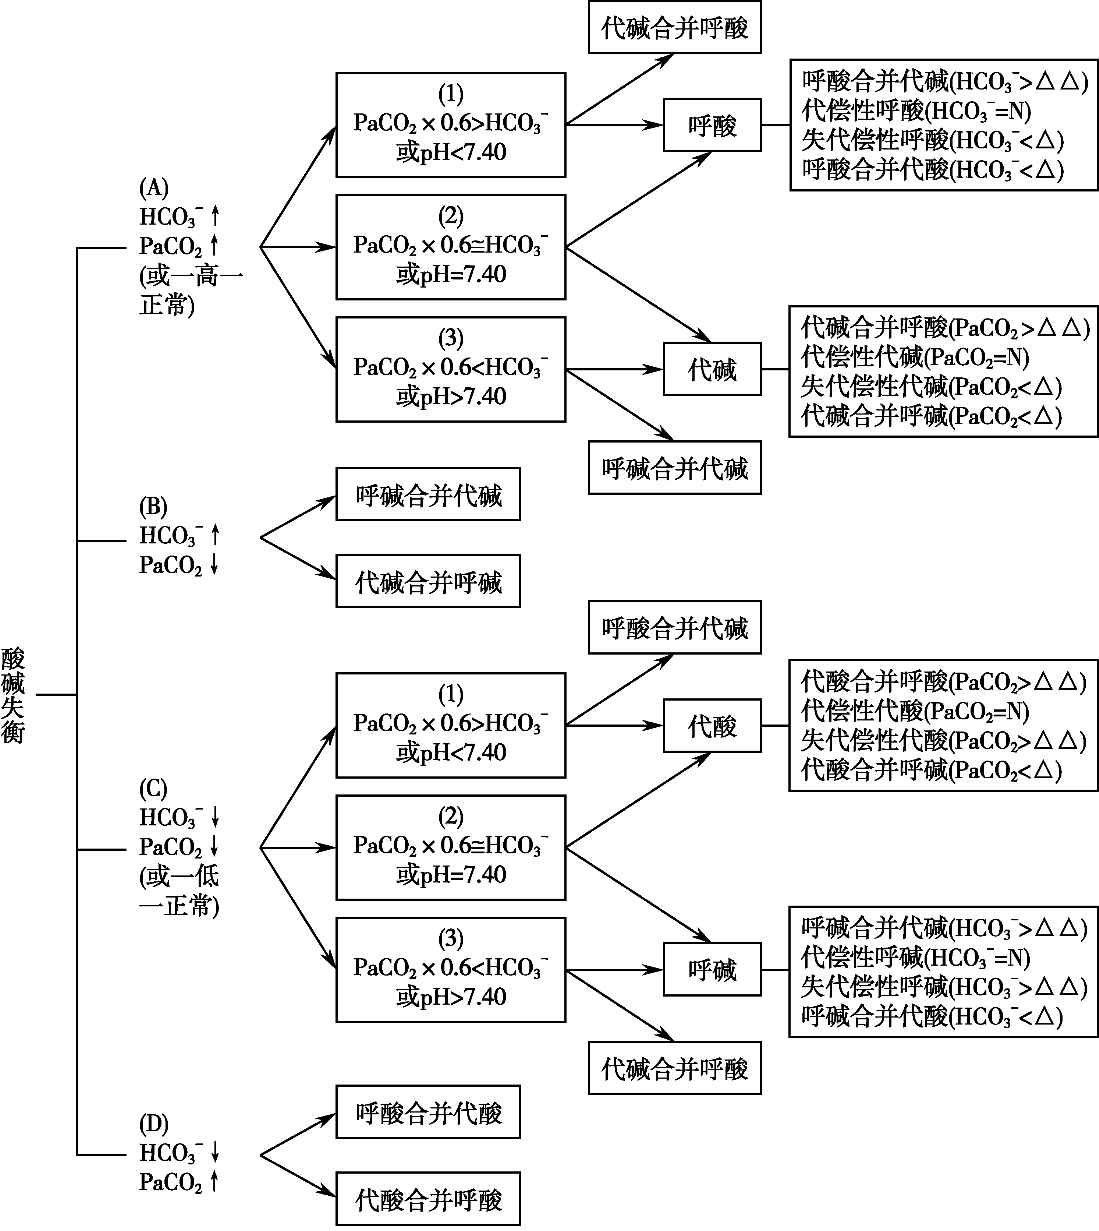
\includegraphics[width=4.97917in,height=5.57292in]{./images/Image00354.jpg}
 \captionsetup{justification=centering}
 \caption{酸碱平衡失调类型筛选判断法}
 \label{fig68-4}
  \end{figure} 

(1) 计算假定无代谢性酸中毒影响的PaCO(\textsubscript{2} NA)= (AG −
12)× 1.2 + PaCO\textsubscript{2}

(2) 计算PaCO(NA)的{} 代偿预计值HCO\textsuperscript{−}

\textsubscript{23} (PNA):如PaCO(\textsubscript{2}
NA)≥40(提示呼吸性酸中毒或正常),
\includegraphics[width=2.5625in,height=0.16667in]{./images/Image00356.jpg}
;如PaCO\textsubscript{2} (NA)<
40(提示呼吸性碱中毒),HCO(\textsuperscript{−} PNA)= 24 −(40 −

\textsubscript{3} PaCO(\textsubscript{2} NA))× 0.5 + 2.5

(3)
计算假定无代谢性酸中毒影响的
\includegraphics[width=0.875in,height=0.15625in]{./images/Image00357.jpg}
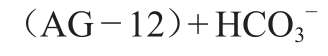
\includegraphics[width=1.08333in,height=0.17708in]{./images/Image00358.jpg}

(4) 比较{}
(NA)与
\includegraphics[width=0.72917in,height=0.13542in]{./images/Image00360.jpg}
,提示无代谢性碱中毒,则最后判断是呼吸性酸中毒+代谢性酸中毒或呼吸性碱中毒+代谢性酸中毒;如
\includegraphics[width=1.5in,height=0.15625in]{./images/Image00361.jpg}
,提示合并代谢性碱中毒或呼吸性碱中毒失代偿两种可能,应根据病史加以确定,最后判断为呼酸型或呼碱型TABD,或呼吸性碱中毒+代谢性酸中毒。

3.如前三步判断为代谢性酸中毒,在AG > 16mmol/L且血Cl\textsuperscript{−}
和(或)血K\textsuperscript{+} 明显减低及(AG − 12)>(24 −{}
)时,可判断代谢性酸中毒合并代谢性碱中毒。

4.如前三步判断是代谢性碱中毒或无酸碱平衡失调,而AG >
16mmol/L,可判断为代谢性酸中毒+代谢性碱中毒,不需考虑TABD。

\protect\hypertarget{text00210.html}{}{}

\hypertarget{text00210.htmlux5cux23CHP6-5-9}{}
参 考 文 献

1. 邦加德(Bongard
FS).现代重症监护诊断与治疗.第2版.北京:人民卫生出版社,2003.

2. Nakal T,Bellomo R. Bench-to-bedside review:Treating acidbase
abnormalities in the intensive care unit- the role of renal replacement
therapy. Critical Care,2004,8:108-114.

3. 韩志钧
,胡成进,黄志锋,等.血气酸碱分析.第2版.沈阳:辽宁科学技术出版社,2006.

\protect\hypertarget{text00211.html}{}{}

